%%%%%%%%%%%%%%%%%%%%%%%%%%%%%%%%%%%%%%%%%%%%%%%%%%%%%%%%%%%%%%%%%%%%%%%%%%%

\documentclass[a4paper,oneside,12pt]{article}
\usepackage{mystyle}

\begin{document}

\title{\Large\bf Trigonometric functions}
\author{%%
  Minh Van Nguyen \\
  \url{mvngu@gmx.com}
}
\date{\today}
\maketitle

\noindent
By now, you should be familiar with the sine function $\sin x$ and the
cosine function $\cos x$, where $x$ is an angle in radians.  In this
document, you will further investigate properties of the sine and
cosine functions.  Trigonometric functions are found in many physical
phenomena.  A common example is sound waves, which can be explained in
terms of a slinky.\footnote{
  See the video at
  \url{https://youtu.be/kxQj-wPePBU}.  Refer also to the slinky
  simulation at
  \url{http://www.physicsclassroom.com/Physics-Interactives/Waves-and-Sound/Slinky-Lab/Slinky-Lab-Interactive}.
}


%%%%%%%%%%%%%%%%%%%%%%%%%%%%%%%%%%%%%%%%%%%%%%%%%%%%%%%%%%%%%%%%%%%%%%%%%%%

\section{Vertical shift of sine function}

\begin{figure}[!htbp]
\centering
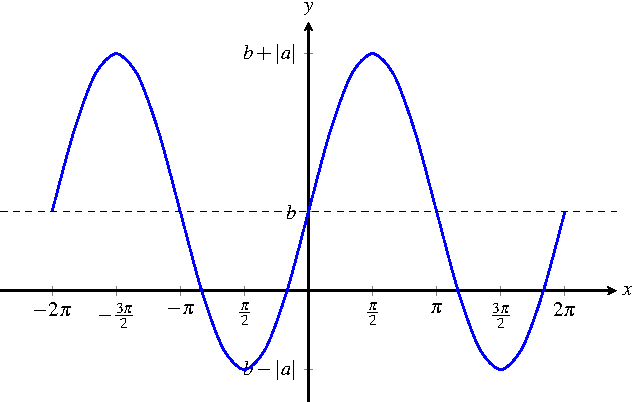
\includegraphics[scale=1.1]{image/13/a-sin-b.pdf}
\caption{%%
  A graph of the general sine function
  $f(x) = a \sin x + b$ from $x = -2\pi$ to $x = 2\pi$.  The midline
  of $f(x)$ is the dashed horizontal line $y = b$.  The amplitude of
  $f(x)$ is the absolute value $\absoluteValue{a}$.
}
\label{fig:trigonometric:general_sine}
\end{figure}

Let $a$ and $b$ be fixed real numbers and let $x$ be a real variable
that represents an angle in radians.  The value of $a$ is often
assumed to be $a \neq 0$.  The sine function can be written
as
\[
f(x)
=
a \sin x + b
\]
which is graphed in \Figure{fig:trigonometric:general_sine}.  The
number $b$ is called the \emph{midline} of $f(x)$ and the absolute
value $\absoluteValue{a}$ is called the \emph{amplitude} of $f(x)$.
The amplitude $\absoluteValue{a}$ measures how high and how low the
value of the sine function $f(x)$ can be.\footnote{
  See the video at
  \url{https://youtu.be/2Kos5VrtTtA}.
}
As you can see in \Figure{fig:trigonometric:general_sine}, given the
sine function $f(x) = a \sin x + b$ the highest value of $f(x)$ is
$b + \absoluteValue{a}$, which is the value of the midline plut the
amplitude.  Furthermore, the lowest value of $f(x)$ is
$b - \absoluteValue{a}$, which is the value of the midline minus the
amplitude.  The number $b$ is the midline of the sine function $f(x)$
because the horizontal line $y = b$ is midway between the highest and
lowest values of $f(x)$.  In fact, if $h$ is the highest value of
$f(x)$ and $\ell$ is the lowest value of $f(x)$, then the value of the
midline is the average $\frac{h + \ell}{2}$.  If you draw the
horizontal line $y = b$ on a graph of $f(x)$~(e.g.~the dashed
horizontal line in \Figure{fig:trigonometric:general_sine}) you will
see that $f(x) = b$ whenever $a \sin x = 0$.  The above is summarised
in \Definition{def:trigonometric:sine_amplitude_and_midline}.

\begin{definition}
\label{def:trigonometric:sine_amplitude_and_midline}
\textbf{Amplitude and midline.}
Let $a$ and $b$ be real constants such that $a \neq 0$.  Given the
sine function $f(x) = a \sin x + b$, the number $\absoluteValue{a}$ is
called the \emph{amplitude} of $f(x)$ and the horizontal line $y = b$
is called the \emph{midline} of $f(x)$.
\end{definition}

\begin{figure}[!htbp]
\centering
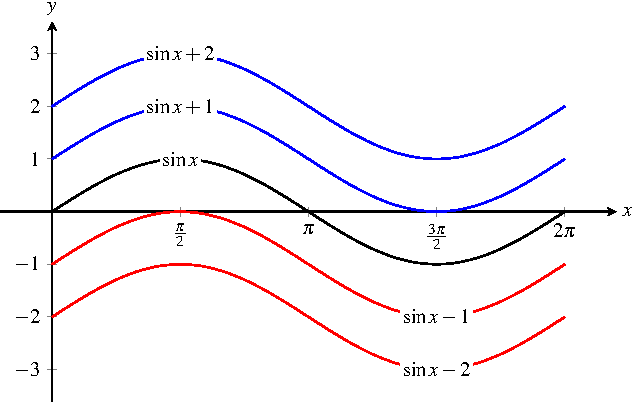
\includegraphics[scale=1.1]{image/13/sin-vertical-shift.pdf}
\caption{%%
  The value of the midline has the effect of vertically shifting the
  graph of the sine function.
}
\label{fig:trigonometric:sine_vertical_shift}
\end{figure}

How does the value of the midline affect the graph of the sine
function?  The value of the midline has the effect of shifting the
graph of the sine function vertically.  If the value of the midline is
positive, i.e.~$b > 0$, then the graph of the sine function will be
shifted upward.  However, if the value of the midline is negative,
i.e.~$b < 0$, then the graph of the sine function will be shifted
downward.  The vertical shift of the sine function is illustrated in
\Figure{fig:trigonometric:sine_vertical_shift}.

\begin{figure}[!htbp]
\centering
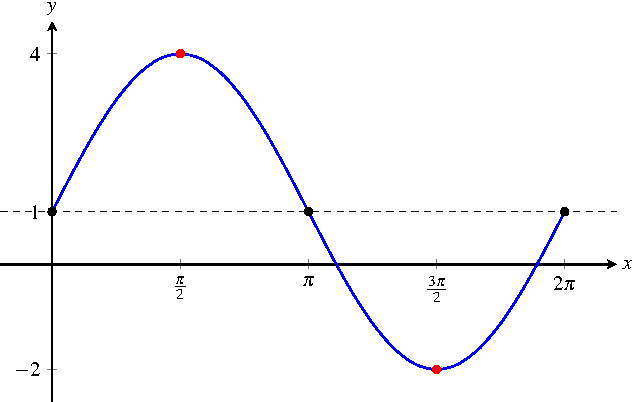
\includegraphics[scale=1.1]{image/13/3-sin-1.pdf}
\caption{%%
  A graph of the sine function $f(x) = 3 \sin x + 1$ from $x = 0$ to
  $x = 2\pi$.
}
\label{fig:trigonometric:sine_3_sin_1}
\end{figure}

\begin{example}
Consider the sine function $f(x) = 3 \sin x + 1$.  Determine the
midline and amplitude of $f(x)$.  Calculate the highest and lowest
values of the function.  Draw a graph of $f(x)$ from $x = 0$ to
$x = 2\pi$.
\end{example}

\begin{solution}
The first thing you should do is work out the midline and amplitude of
the function $f(x)$.  The midline of the function is $y = 1$.  The
amplitude is $3$.  The highest value of $f(x)$ is obtained by adding
the amplitude $3$ to the value of the midline.  Doing so gives you the
value $1 + 3 = 4$.  The lowest value of $f(x)$ is obtained by
subtracting the amplitude $3$ from the value of the midline.  Doing so
results in $1 - 3 = -2$.  Thus the highest value of $f(x)$ is $4$ and
the lowest value of $f(x)$ is $-2$.
\Figure{fig:trigonometric:sine_3_sin_1} shows the midline $y = 1$ as a
dashed horizontal line.

Next, determine all values of $x$ within the range
$0 \leq x \leq 2\pi$ such that the graph of $f(x)$ intersects the
midline.  This is equivalent to determining all values of $x$ such
that $\sin x = 0$.  The reason is that if $\sin x = 0$, then the
function $f(x) = 3 \sin x + 1$ simplifies to $f(x) = 1$, which is the
midline.  You know that $\sin x = 0$ when
$x = \triple{0}{\pi}{2\pi}$ and so you have
$f(0) = f(\pi) = f(2\pi) = 3 \times 0 + 1 = 1$.  In other words, the
graph of $f(x)$ intersects the midline $y = 1$ at the points
$\tuple{0}{1}$, $\tuple{\pi}{1}$, and $\tuple{2\pi}{1}$.
\Figure{fig:trigonometric:sine_3_sin_1} shows the points of
intersection as black dots.

Now determine the highest and lowest points of $f(x)$, where
$0 \leq x \leq 2\pi$.  To determine the highest point of $f(x)$, you
determine the highest value of $\sin x$.  You know that the highest
value of $\sin x$ is $1$, which occurs when $x = \frac{\pi}{2}$.  Then
the highest value of $f(x)$ is $f(\pi/2) = 3 \times 1 + 1 = 4$ so that
the highest point of $f(x)$ is $\tuple{\frac{\pi}{2}}{4}$.  Similarly,
the lowest value of $\sin x$ is $-1$, which occurs when
$x = \frac{3\pi}{2}$.  Then the lowest value of $f(x)$ is
$f(3\pi/2) = 3(-1) + 1 = -2$ so that the lowest point of $f(x)$ is
$\tuple{\frac{3\pi}{2}}{-2}$.  The highest and lowest points of $f(x)$
are shown in \Figure{fig:trigonometric:sine_3_sin_1} as red dots.

Finally, draw a wave through the above five points and you obtain the
graph in \Figure{fig:trigonometric:sine_3_sin_1}.
\end{solution}

\begin{exercise}
Consider the function $f(x) = 4 \sin x + 2$.  Determine the midline
and amplitude of $f(x)$.  Calculate the highest and lowest values of
the function.  Draw a graph of $f(x)$ from $x = 0$ to $x = 2\pi$.
\end{exercise}

\ifbool{showSolution}{
\begin{solution}
The midline of $f(x)$ is the horizontal line $y = 2$.  The amplitude
of $f(x)$ is $4$.  To obtain the highest value of $f(x)$, you add the
amplitude $4$ to the value of the midline and get $2 + 4 = 6$.  To
obtain the lowest value of $f(x)$, you subtract the amplitude $4$ from
the value of the midline and get $2 - 4 = -2$.  That is, the highest
and lowest values of $f(x)$ are $6$ and $-2$, respectively.

To graph $f(x)$ from $x = 0$ to $x = 2\pi$, you should first determine
those values of $x$ for which the graph of $f(x)$ intersects the
midline.  This is the same as determining all values of $x$ such that
$\sin x = 0$.  You know that $\sin 0 = \sin \pi = \sin 2\pi = 0$ so
that when $x = \triple{0}{\pi}{2\pi}$ you have
$f(0) = f(\pi) = f(2\pi) = 4 \times 0 + 2 = 2$.  Thus the graph of
$f(x)$ intersects the midline at the points $\tuple{0}{2}$,
$\tuple{\pi}{2}$, and $\tuple{2\pi}{2}$.

Next, you determine the highest and lowest points of $f(x)$ within the
range $0 \leq x \leq 2\pi$.  You know that the highest value of
$\sin x$ is $1$, which occurs when $x = \frac{\pi}{2}$.  Substitute
the latter value into $f(x)$ and you obtain
%%
\begin{align*}
f(\pi/2)
&=
4 \sin \frac{\pi}{2} + 2 \\[4pt]
&=
4 \times 1 + 2 \\[4pt]
&=
6.
\end{align*}
%%
The lowest value of $\sin x$ is $-1$, which occurs when
$x = \frac{3\pi}{2}$.  Substitute the latter value into the function
$f(x)$ and simplify to obtain
%%
\begin{align*}
f(3\pi / 2)
&=
4 \sin \frac{3\pi}{2} + 2 \\[4pt]
&=
4 (-1) + 2 \\[4pt]
&=
-4 + 2 \\[4pt]
&=
-2.
\end{align*}
%%
In other words, the highest point of $f(x)$ is
$\tuple{\frac{\pi}{2}}{6}$ and the lowest point of $f(x)$ is
$\tuple{\frac{3\pi}{2}}{-2}$.

\begin{figure}[!htbp]
\centering
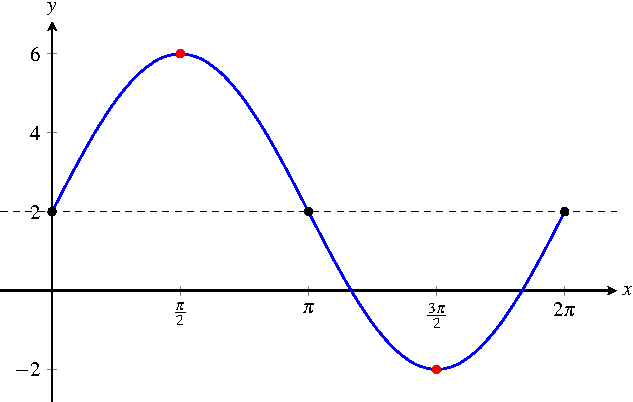
\includegraphics[scale=1.1]{image/13/4-sin-2.pdf}
\caption{%%
  A graph of the function $f(x) = 4 \sin x + 2$ from $x = 0$ to
  $x = 2\pi$.
}
\label{fig:trigonometric:4_sinx_2}
\end{figure}

Finally, draw a wave through the above points and you obtain the graph
shown in \Figure{fig:trigonometric:4_sinx_2}.  The black dots show the
points at which the graph of $f(x)$ intersects the midline $y = 2$.
The red dots show the highest and lowest points of $f(x)$.
\end{solution}
}{}

\begin{exercise}
Consider the function $f(x) = -2 \sin x + 6$.  Determine the midline
and amplitude of $f(x)$.  Calculate the highest and lowest values of
the function.  Draw a graph of $f(x)$ from $x = 0$ to $x = 2\pi$.
\end{exercise}

\ifbool{showSolution}{
\begin{solution}
The midline of the function $f(x)$ is $y = 6$ and the amplitude is
$\absoluteValue{-2} = 2$.  \Figure{fig:trigonometric:minus2_sin_6}
shows the midline as a dashed horizontal line.  The highest value of
$f(x)$ is obtained by adding the amplitude to the value of the
midline.  Then the required highest value is $6 + 2 = 8$.  Similarly,
the lowest value of $f(x)$ is obtained by subtracting the amplitude
from the value of the midline.  Thus the lowest value of $f(x)$ is
$6 - 2 = 4$.

\begin{figure}[!htbp]
\centering
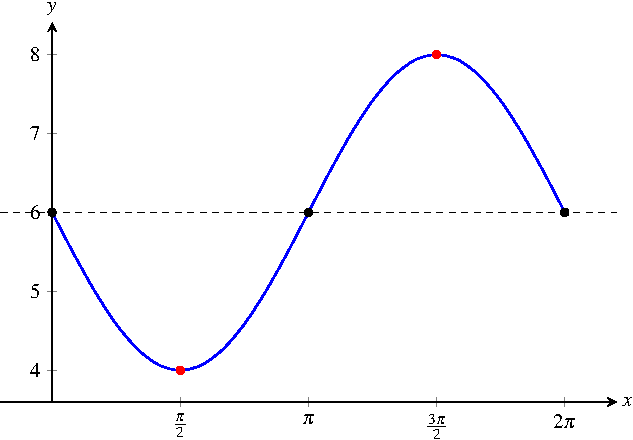
\includegraphics[scale=1.1]{image/13/minus2-sin-6.pdf}
\caption{%%
  A graph of the function $f(x) = -2 \sin x + 6$ from $x = 0$ to
  $x = 2\pi$.
}
\label{fig:trigonometric:minus2_sin_6}
\end{figure}

To draw a graph of the function $f(x)$ within the range
$0 \leq x \leq 2\pi$, you should first determine all points of $f(x)$
at which the graph of $f(x)$ intersects the midline.  This is the same
as determining all values of $x$ such that $\sin x = 0$.  You already
know that $\sin x = 0$ whenever $x = \triple{0}{\pi}{2\pi}$.  Then you
have $f(0) = f(\pi) = f(2\pi) = 6$.  In other words, the graph of
$f(x)$ intersects the midline at the points $\tuple{0}{6}$,
$\tuple{\pi}{6}$, and $\tuple{2\pi}{6}$.  The points of intersection
are shown in \Figure{fig:trigonometric:minus2_sin_6} as black dots.

Next, determine the highest and lowest points of $f(x)$.  Note that
the highest value of $\sin x$ is $1$, which occurs when
$x = \frac{\pi}{2}$.  Then $f(\pi/2) = -2 \times 1 + 6 = 4$, which is
the lowest value of $f(x)$.  That is, the lowest point of $f(x)$ is
$\tuple{\frac{\pi}{2}}{4}$.  Furthermore, the lowest value of $\sin x$
is $-1$, which occurs when $x = \frac{3\pi}{2}$.  Then you have
$f(3\pi/2) = -2 (-1) + 6 = 8$, which is the highest value of $f(x)$.
The highest point of $f(x)$ is $\tuple{\frac{3\pi}{2}}{8}$.  The
highest and lowest points are shown in
\Figure{fig:trigonometric:minus2_sin_6} as red dots.

Finally, draw a wave through the five points to obtain the graph shown
in \Figure{fig:trigonometric:minus2_sin_6}.
\end{solution}
}{}

\begin{figure}[!htbp]
\centering
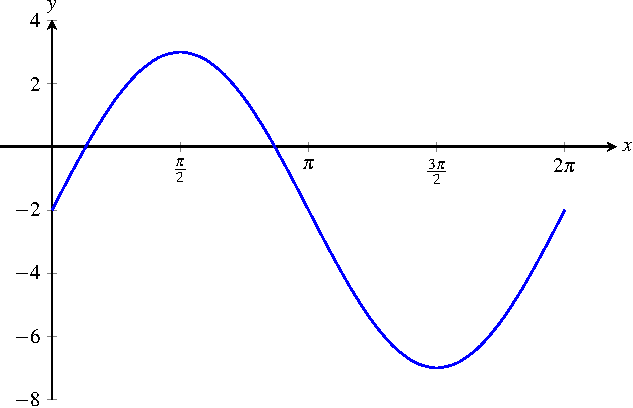
\includegraphics[scale=1.1]{image/13/5-sin-minus2.pdf}
\caption{%%
  A graph of a sine function of the form $f(x) = a \sin x + b$ from
  $x = 0$ to $x = 2\pi$.
}
\label{fig:trigonometric:5_sin_minus2}
\end{figure}

\begin{exercise}
\Figure{fig:trigonometric:5_sin_minus2} shows a graph of a sine
function that has a midline of $y = -2$.  The function has
$\tuple{\frac{\pi}{2}}{3}$ as one of its highest points.  If the
function is of the form $f(x) = a \sin x + b$, determine the values of
$a$ and $b$.
\end{exercise}

\ifbool{showSolution}{
\begin{solution}
Since the midline is $y = -2$, then $b = -2$.  The highest value of
$f(x)$ is obtained by adding the amplitude to the value of the
midline.  If the amplitude is $a$, then you have the equation
$-2 + a = 3$.  Solving the latter equation for $a$ yields
%%
\begin{align*}
a
&=
3 + 2 \\[4pt]
&=
5.
\end{align*}
%%
In other words, the amplitude is $a = 5$.  Therefore,
\Figure{fig:trigonometric:5_sin_minus2} shows a graph of the function
$f(x) = 5 \sin x - 2$.
\end{solution}
}{}

\begin{exercise}
A sine function $f(x) = a \sin x + b$ has
$\tuple{\frac{\pi}{2}}{\frac{15}{2}}$ and
$\tuple{\frac{3\pi}{2}}{-\frac{1}{2}}$ as some of its highest and
lowest points, respectively.  Determine the amplitude and midline of
$f(x)$.  Sketch a graph of $f(x)$ from $x = 0$ to $x = 2\pi$.
\end{exercise}

\ifbool{showSolution}{
\begin{solution}
Since $\frac{15}{2}$ is the highest value of $f(x)$ and $-\frac{1}{2}$
is the lowest value of $f(x)$, then the value of the midline is the
average of the highest and lowest values.  Thus the midline of $f(x)$
is
%%
\begin{align*}
y
&=
\frac{1}{2} \parenthesis*{\frac{15}{2} - \frac{1}{2}} \\[4pt]
&=
\frac{1}{2} \parenthesis*{\frac{15 - 1}{2}} \\[4pt]
&=
\frac{1}{2} \times 7 \\[4pt]
&=
\frac{7}{2}.
\end{align*}
%%
The amplitude of $f(x)$ is the difference between the highest value of
$f(x)$ and the value of the midline.  The amplitude is also the
difference between the value of the midline and the lowest value of
$f(x)$.  That is, the amplitude of $f(x)$ is
%%
\begin{align*}
a
&=
\frac{15}{2} - \frac{7}{2} \\[4pt]
&=
\frac{15 - 7}{2} \\[4pt]
&=
\frac{8}{2} \\[4pt]
&=
4.
\end{align*}
%%
Thus the function $f(x)$ can be written as
$f(x) = 4 \sin x + \frac{7}{2}$ and is graphed in
\Figure{fig:trigonometric:4_sin_7half}.

\begin{figure}[!htbp]
\centering
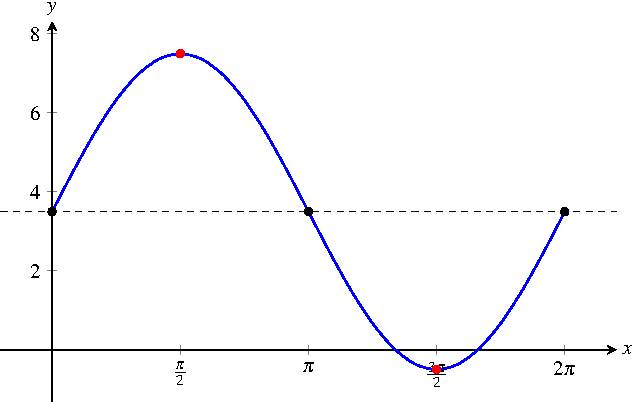
\includegraphics[scale=1.1]{image/13/4-sin-7half.pdf}
\caption{%%
  A graph of the function $f(x) = 4 \sin x + \frac{7}{2}$ from
  $x = 0$ to $x = 2\pi$.
}
\label{fig:trigonometric:4_sin_7half}
\end{figure}

\end{solution}
}{}

\begin{exercise}
Consider the function $f(x) = a \sin x$.  Graph the function when
$a = \triple{1}{\frac{3}{2}}{2}$.  Also graph the function when
$a = \triple{1}{\frac{1}{2}}{\frac{3}{4}}$.  Describe the effect of
the value of the amplitude on the graph of the sine function.
\end{exercise}

\ifbool{showSolution}{
\begin{solution}
\Figures{fig:trigonometric:sine_vertical_stretch}{fig:trigonometric:sine_vertical_compress}
show graphs of the function $f(x) = a \sin x$ when the values of the
amplitude are $a = \triple{1}{\frac{3}{2}}{2}$ and
$a = \triple{1}{\frac{3}{4}}{\frac{1}{2}}$.  As the figures show, when
the amplitude is $a > 1$, the graph of the sine function is stretched
in the vertical direction.  When the amplitude is $0 < a < 1$, the
graph of the sine function is compressed in the vertical direction.

\begin{figure}[!htbp]
\centering
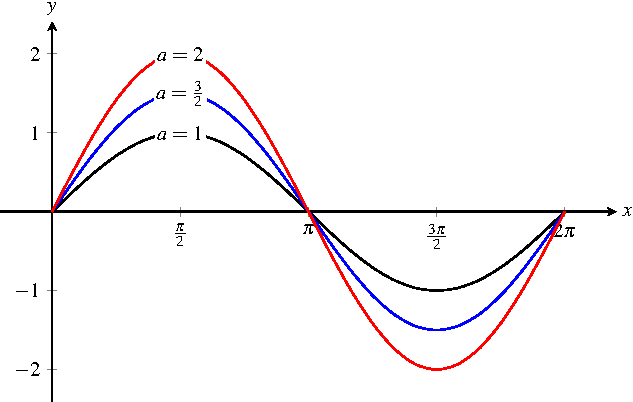
\includegraphics[scale=1.1]{image/13/sin-vertical-stretch.pdf}
\caption{%%
  Graphs of the function $f(x) = a \sin x$ for
  $a = \triple{1}{\frac{3}{2}}{2}$.
}
\label{fig:trigonometric:sine_vertical_stretch}
\end{figure}

\begin{figure}[!htbp]
\centering
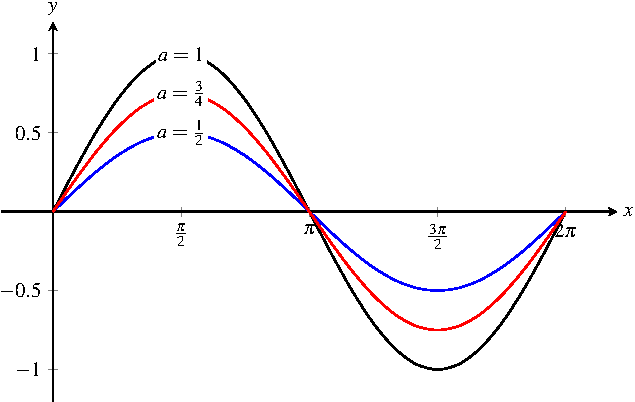
\includegraphics[scale=1.1]{image/13/sin-vertical-compress.pdf}
\caption{%%
  Graphs of the function $f(x) = a \sin x$ for
  $a = \triple{1}{\frac{3}{4}}{\frac{1}{2}}$.
}
\label{fig:trigonometric:sine_vertical_compress}
\end{figure}

\end{solution}
}{}


%%%%%%%%%%%%%%%%%%%%%%%%%%%%%%%%%%%%%%%%%%%%%%%%%%%%%%%%%%%%%%%%%%%%%%%%%%%

\section{Vertical shift of cosine function}

Let $a$ and $b$ be fixed real numbers such that $a \neq 0$ and let $x$
be a real variable.  The cosine function can be written as
\[
f(x)
=
a \cos x + b
\]
and is graphed in \Figure{fig:trigonometric:a_cos_b} from $x = -2\pi$
to $x = 2\pi$.  The \emph{midline} of $f(x)$ is the horizontal line
$y = b$.  The \emph{amplitude} of $f(x)$ is the absolute value
$\absoluteValue{a}$.  The highest value of $f(x)$ is obtained by
adding the amplitude to the value of the midline.  Similarly, the
lowest value of $f(x)$ is obtained by subtracting the amplitude from
the value of the midline. Thus the highest value of $f(x)$ is
$b + \absoluteValue{a}$ and the lowest value of $f(x)$ is
$b - \absoluteValue{a}$.  The value $b$ of the midline is halfway
between the highest and lowest values of $f(x)$.  If $h$ is the
highest value of $f(x)$ and $\ell$ is the lowest value of $f(x)$, then
the value of the midline is the average $\frac{h + \ell}{2}$.  The
above is summarised in
\Definition{def:trigonometric:cosine_amplitude_and_midline}.

\begin{definition}
\label{def:trigonometric:cosine_amplitude_and_midline}
\textbf{Amplitude and midline.}
Let $a$ and $b$ be real constants such that $a \neq 0$.  Given the
cosine function $f(x) = a \cos x + b$, the number $\absoluteValue{a}$
is called the \emph{amplitude} of $f(x)$ and the horizontal line $y =
b$ is called the \emph{midline} of $f(x)$.
\end{definition}

\begin{figure}[!htbp]
\centering
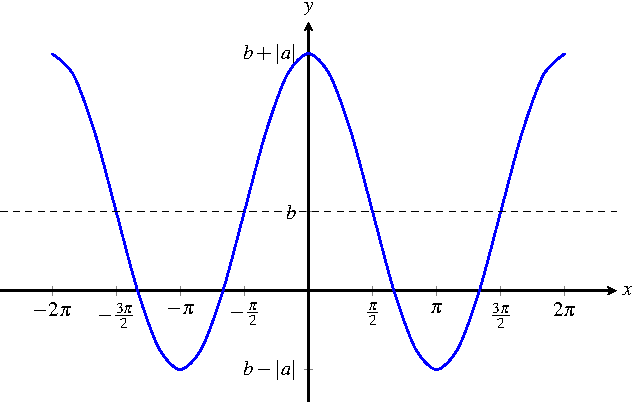
\includegraphics[scale=1.1]{image/13/a-cos-b.pdf}
\caption{%%
  A graph of the general cosine function $f(x) = a \cos x + b$ from
  $x = -2\pi$ to $x = 2\pi$.  The midline of $f(x)$ is the dashed
  horizontal line $y = b$.  The amplitude of $f(x)$ is the absolute
  value $\absoluteValue{a}$.
}
\label{fig:trigonometric:a_cos_b}
\end{figure}

Just as the value of the midline vertically shifts the graph of a sine
function, the value of the midline also vertically shifts the graph of
a cosine function.  If the value of the midline is positive,
i.e.~$b > 0$, then the graph of the cosine function will be shifted
upward.  On the other hand, if the value of the midline is negative,
i.e.~$b < 0$, the graph of the cosine function will be shifted
downward.  \Figure{fig:trigonometric:cos_vertical_shift} illustrates
the vertical shift of the graph of the cosine function.

\begin{figure}[!htbp]
\centering
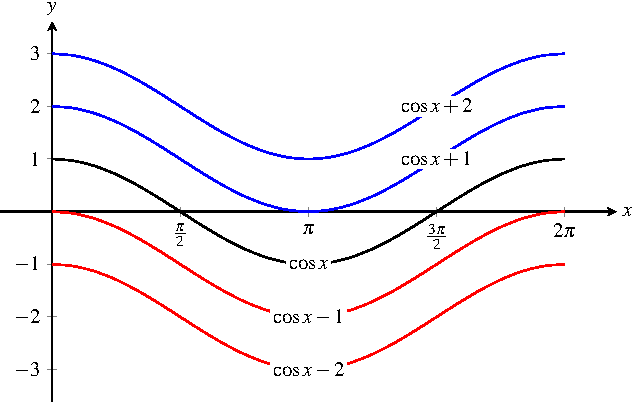
\includegraphics[scale=1.1]{image/13/cos-vertical-shift.pdf}
\caption{%%
  The value of the midline has the effect of vertically shifting the
  graph of the cosine function.
}
\label{fig:trigonometric:cos_vertical_shift}
\end{figure}

\begin{figure}[!htbp]
\centering
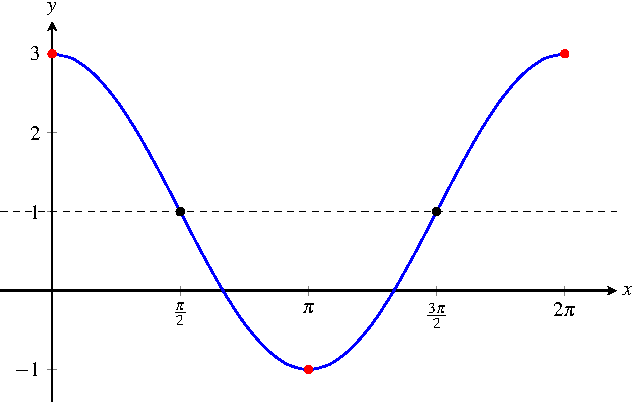
\includegraphics[scale=1.1]{image/13/2-cos-3.pdf}
\caption{%%
  A graph of the function $f(x) = 2 \cos x + 1$ from $x = 0$ to
  $x = 2\pi$.
}
\label{fig:trigonometric:2_cos_1}
\end{figure}

\begin{example}
Consider the function $f(x) = 2 \cos x + 1$.  Determine the midline
and amplitude of $f(x)$.  Calculate the highest and lowest values of
the function.  Sketch a graph of $f(x)$ from $x = 0$ to $x = 2\pi$.
\end{example}

\begin{solution}
The midline of the function $f(x)$ is $y = 1$ and the amplitude is
$2$.  The midline is shown in \Figure{fig:trigonometric:2_cos_1} as a
dashed horizontal line.  The highest value of $f(x)$ is obtained by
adding the amplitude to the value of the midline.  Thus the highest
value of $f(x)$ is $1 + 2 = 3$.  The lowest value of $f(x)$ is
obtained by subtracting the amplitude from the value of the midline.
Then the lowest value of $f(x)$ is $1 - 2 = -1$.

To sketch a graph of $f(x)$ from $x = 0$ to $x = 2\pi$, you should
first determine all points of $f(x)$ at which the graph of $f(x)$
intersects the midline $y = 1$.  That is, you want all values of $x$
such that $\cos x = 0$.  The reason is that if $\cos x = 0$ then
$f(x)$ simplifies to $f(x) = 1$, which is $y$-coordinate of the
midline.  You know that $\cos x = 0$ whenever
$x = \pair{\frac{\pi}{2}}{\frac{3\pi}{2}}$.  Then the graph of $f(x)$
intersects the midline at the points $\tuple{\frac{\pi}{2}}{1}$ and
$\tuple{\frac{3\pi}{2}}{1}$.  The points of intersection are shown in
\Figure{fig:trigonometric:2_cos_1} as black dots.

Next, you should determine the highest and lowest points of $f(x)$.
The highest value of $\cos x$ is $1$, which occurs whenever
$x = \pair{0}{2\pi}$.  Then you have
$f(0) = f(2\pi) = 2 \times 1 + 1 = 3$, which is the highest value of
$f(x)$.  Thus the highest points of $f(x)$ are $\tuple{0}{3}$ and
$\tuple{2\pi}{3}$.  Furthermore, the lowest value of $\cos x$ is $-1$,
which occurs whenever $x = \pi$.  Then you have
$f(\pi) = 2 (-1) + 1 = -1$, which is the lowest value of $f(x)$.  Thus
the lowest point of $f(x)$ is $\tuple{\pi}{-1}$.  The highest and
lowest points of $f(x)$ are shown in
\Figure{fig:trigonometric:2_cos_1} as red dots.

Finally, draw a wave through the five points above to obtain the graph
shown in \Figure{fig:trigonometric:2_cos_1}.
\end{solution}

\begin{exercise}
Consider the function $f(x) = \frac{3}{2} \cos x - 1$.  Determine the
midline and amplitude of the function.  Calculate the highest and
lowest values of $f(x)$.  Sketch a graph of $f(x)$ from $x = 0$ to
$x = 2\pi$.
\end{exercise}

\ifbool{showSolution}{
\begin{solution}
The function $f(x)$ has a midline of $y = -1$ and an amplitude of
$3/2$.  \Figure{fig:trigonometric:3half_cos_minus1} shows the midline
as a dashed horizontal line.  The highest value of $f(x)$ is obtained
by adding the amplitude to the value of the midline.  That is, the
highest value of $f(x)$ is
%%
\begin{align*}
-1 + \frac{3}{2}
&=
\frac{-2}{2} + \frac{3}{2} \\[4pt]
&=
\frac{-2 + 3}{2} \\[4pt]
&=
\frac{1}{2}.
\end{align*}
%%
The lowest value of $f(x)$ is obtained by subtracting the amplitude
from the value of the midline.  In other words, the lowest value of
$f(x)$ is
%%
\begin{align*}
-1 - \frac{3}{2}
&=
\frac{-2}{2} - \frac{3}{2} \\[4pt]
&=
\frac{-2 - 3}{2} \\[4pt]
&=
-\frac{5}{2}.
\end{align*}

\begin{figure}[!htbp]
\centering
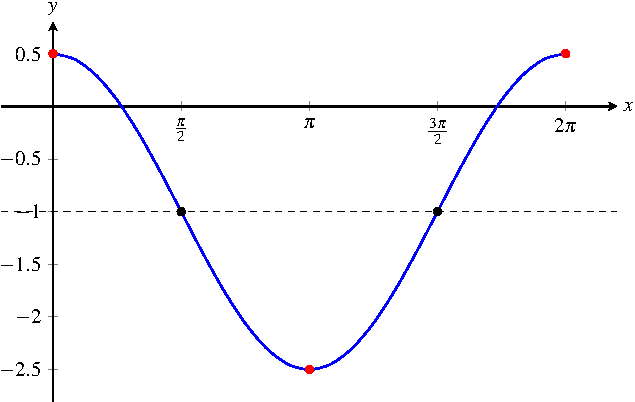
\includegraphics[scale=1.1]{image/13/3half-cos-minus1.pdf}
\caption{%%
  A graph of the function $f(x) = \frac{3}{2} \cos x - 1$ from $x = 0$
  to $x = 2\pi$.
}
\label{fig:trigonometric:3half_cos_minus1}
\end{figure}

To sketch a graph of $f(x)$ from $x = 0$ to $x = 2\pi$, first you
should determine all points at which the graph of $f(x)$ intersects
the midline.  This is the same as determining all values of $x$ such
that $\cos x = 0$.  You know that $\cos x = 0$ whenever
$x = \pair{\frac{\pi}{2}}{\frac{3\pi}{2}}$ and so you have
$f(\pi/2) = f(3\pi/2) = \frac{3}{2} \times 0 - 1 = -1$.  Thus the
graph of $f(x)$ intersects the midline at the points
$\tuple{\frac{\pi}{2}}{-1}$ and $\tuple{\frac{3\pi}{2}}{-1}$.  The
points of intersection are shown in
\Figure{fig:trigonometric:3half_cos_minus1} as black dots.

Next, you determine the highest and lowest points of $f(x)$.  The
highest value of $\cos x$ is $1$, which occurs whenever
$x = \pair{0}{2\pi}$.  Then you have
$f(0) = f(2\pi) = \frac{3}{2} \times 1 - 1 = \frac{1}{2}$.  The lowest
value of $\cos x$ is $-1$, which occurs whenever $x = \pi$.  Then you
have $f(\pi) = \frac{3}{2} (-1) - 1 = -\frac{5}{2}$.  In other words,
the highest points of $f(x)$ are $\tuple{0}{\frac{1}{2}}$ and
$\tuple{2\pi}{\frac{1}{2}}$.  The lowest point of $f(x)$ is
$\tuple{\pi}{-\frac{5}{2}}$.  The highest and lowest points are shown
in \Figure{fig:trigonometric:3half_cos_minus1} as red dots.

Finally, draw a wave through the above five points and you obtain the
graph in \Figure{fig:trigonometric:3half_cos_minus1}.
\end{solution}
}{}

\begin{exercise}
Consider the function $f(x) = -4 \cos x + 3$.  Determine the midline
and amplitude of $f(x)$.  Calculate the highest and lowest values of
the function.  Draw a graph of $f(x)$ from $x = 0$ to $x = 2\pi$.
\end{exercise}

\ifbool{showSolution}{
\begin{solution}
The midline of the function $f(x)$ is $y = 3$, which is shown in
\Figure{fig:trigonometric:minus4_cos_3} as a dashed horizontal line.
The amplitude of the function is the absolute value
$\absoluteValue{-4} = 4$.  The highest value of $f(x)$ is obtained by
adding the amplitude to the value of the midline.  Thus the highest
value of $f(x)$ is $3 + 4 = 7$.  The lowest value of $f(x)$ is
obtained by subtracting the amplitude from the value of the midline.
That is, the lowest value of $f(x)$ is $3 - 4 = -1$.

\begin{figure}[!htbp]
\centering
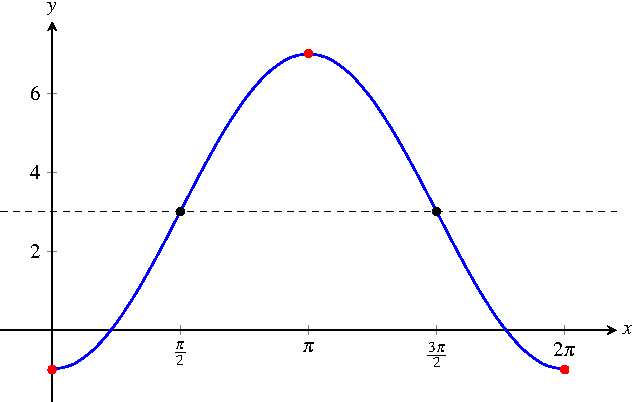
\includegraphics[scale=1.1]{image/13/minus4-cos-3.pdf}
\caption{%%
  A graph of the function $f(x) = -4 \cos x + 3$ from $x = 0$ to
  $x = 2\pi$.
}
\label{fig:trigonometric:minus4_cos_3}
\end{figure}

To draw a graph of $f(x)$ from $x = 0$ to $x = 2\pi$, you should first
determine all points at which the graph of $f(x)$ intersects the
midline.  This occurs for all values of $x$ such that $\cos x = 0$
because if $\cos x = 0$ then the function $f(x)$ simplifies to
$f(x) = 3$, which is the value of the midline.  You know that
$\cos x = 0$ whenever $x = \pair{\frac{\pi}{2}}{\frac{3\pi}{2}}$.
Then you have $f(\pi/2) = f(3\pi/2) = -4 \times 0 + 3 = 3$ and so the
graph of $f(x)$ intersects the midline at the points
$\tuple{\frac{\pi}{2}}{3}$ and $\tuple{\frac{3\pi}{2}}{3}$.  The
points of intersection are shown in
\Figure{fig:trigonometric:minus4_cos_3} as black dots.

Next, you should determine the highest and lowest points of $f(x)$.
Note that the highest value of $\cos x$ is $1$, which occurs whenever
$x = \pair{0}{2\pi}$.  Then you have
$f(0) = f(2\pi) = -4 \times 1 + 3 = -1$, which is the lowest value of
$f(x)$.  Thus the lowest points of $f(x)$ are $\tuple{0}{-1}$ and
$\tuple{2\pi}{-1}$.  Furthermore, the lowest value of $\cos x$ is
$-1$, which occurs whenever $x = \pi$.  Then you have
$f(\pi) = -4 (-1) + 3 = 7$, which is the highest value of $f(x)$.  In
other words, the highest point of $f(x)$ is $\tuple{\pi}{7}$.  The
highest and lowest points of $f(x)$ are shown in
\Figure{fig:trigonometric:minus4_cos_3} as red dots.

Finally, draw a wave through the above five points and you obtain the
graph shown in \Figure{fig:trigonometric:minus4_cos_3}.
\end{solution}
}{}

\begin{figure}[!htbp]
\centering
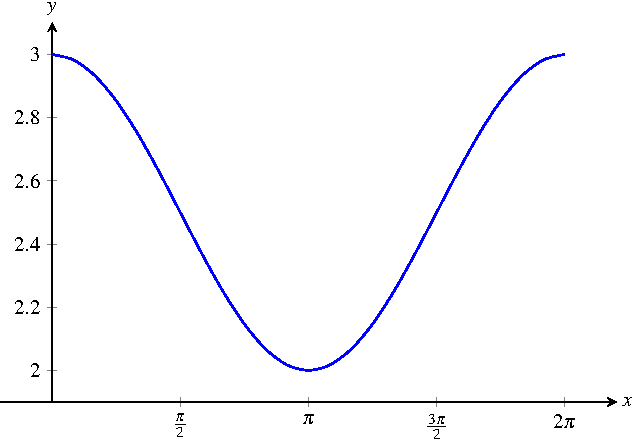
\includegraphics[scale=1.1]{image/13/half-cos-5half.pdf}
\caption{%%
  A graph of a cosine function of the form $f(x) = a \cos x + b$ from
  $x = 0$ to $x = 2\pi$.
}
\label{fig:trigonometric:half_cos_5half}
\end{figure}

\begin{exercise}
\Figure{fig:trigonometric:half_cos_5half} shows a graph of a cosine
function, whose midline is $y = 5/2$.  The function has $\tuple{0}{3}$
as one of its highest points.  If the function is of the form
$f(x) = a \cos x + b$, determine the values of $a$ and $b$.
\end{exercise}

\ifbool{showSolution}{
\begin{solution}
Since the midline is $y = 5/2$, then you have $b = 5/2$.  To get the
highest value of the function, you add the amplitude to the value of
the midline.  If the amplitude is $a$, then you have the equation
$\frac{5}{2} + a = 3$.  Solving the latter equation for $a$ shows that
%%
\begin{align*}
a
&=
3 - \frac{5}{2} \\[4pt]
&=
\frac{6}{2} - \frac{5}{2} \\[4pt]
&=
\frac{6 - 5}{2} \\[4pt]
&=
\frac{1}{2}.
\end{align*}
%%
In other words, the amplitude is $1/2$.  Thus
\Figure{fig:trigonometric:half_cos_5half} shows a graph of the
function $f(x) = \frac{1}{2} \cos x + \frac{5}{2}$.
\end{solution}
}{}

\begin{exercise}
A cosine function $f(x) = a \cos x + b$ has $\tuple{0}{\frac{11}{2}}$
and $\tuple{\pi}{\frac{1}{2}}$ as some of its highest and lowest
points, respectively.  Determine the amplitude and midline of $f(x)$.
Sketch a graph of $f(x)$ from $x = 0$ to $x = 2\pi$.
\end{exercise}

\ifbool{showSolution}{
\begin{solution}
The highest and lowest values of $f(x)$ are $\frac{11}{2}$ and
$\frac{1}{2}$, respectively.  The value of the midline of $f(x)$ is
the average of the highest and lowest values of $f(x)$.  Thus the
midline of $f(x)$ is
%%
\begin{align*}
y
&=
\frac{1}{2} \parenthesis*{\frac{11}{2} + \frac{1}{2}} \\[4pt]
&=
\frac{1}{2} \parenthesis*{\frac{11 + 1}{2}} \\[4pt]
&=
\frac{1}{2} \times 6 \\[4pt]
&=
3.
\end{align*}
%%
The amplitude of $f(x)$ is the difference between the highest value of
$f(x)$ and the value of the midline.  The amplitude can also be
calculated as the difference between the value of the midline and the
lowest value of $f(x)$.  That is, the amplitude of $f(x)$ is
%%
\begin{align*}
\frac{11}{2} - 3
&=
\frac{11}{2} - \frac{6}{2} \\[4pt]
&=
\frac{11 - 6}{2} \\[4pt]
&=
\frac{5}{2}.
\end{align*}
%%
Then the function $f(x)$ can be written as
$f(x) = \frac{5}{2} \cos x + 3$, which is graphed in
\Figure{fig:trigonometric:5half_cos_3}.

\begin{figure}[!htbp]
\centering
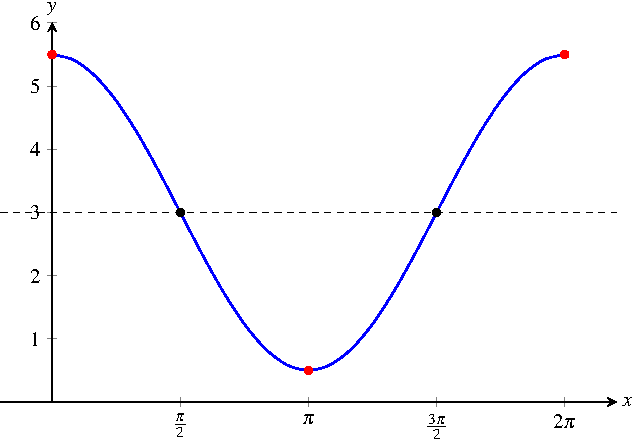
\includegraphics[scale=1.1]{image/13/5half-cos-3.pdf}
\caption{%%
  A graph of the function $f(x) = \frac{5}{2} \cos x + 3$ from $x = 0$
  to $x = 2\pi$.
}
\label{fig:trigonometric:5half_cos_3}
\end{figure}

\end{solution}
}{}

\begin{exercise}
Consider the function $f(x) = a \cos x$.  Graph the function for
$a = \triple{1}{\frac{3}{2}}{2}$.  Also graph the function for
$a = \triple{1}{\frac{1}{2}}{\frac{3}{4}}$.  Describe the effect of
the value of the amplitude on the graph of the cosine function.
\end{exercise}

\ifbool{showSolution}{
\begin{solution}
\Figures{fig:trigonometric:cos_vertical_stretch}{fig:trigonometric:cos_vertical_compress}
show graphs of the function $f(x) = a \cos x$ for
$a = \triple{1}{\frac{3}{2}}{2}$ and for
$a = \triple{1}{\frac{1}{2}}{\frac{3}{4}}$.  When the amplitude is
$a > 1$, the graph of the cosine function is stretched vertically.
However, when the amplitude is $0 < a < 1$, the graph of the cosine
function is compressed vertically.  That is, the value of the
amplitude has the effect of stretching or compressing in the vertical
direction the graph of the cosine function.

\begin{figure}[!htbp]
\centering
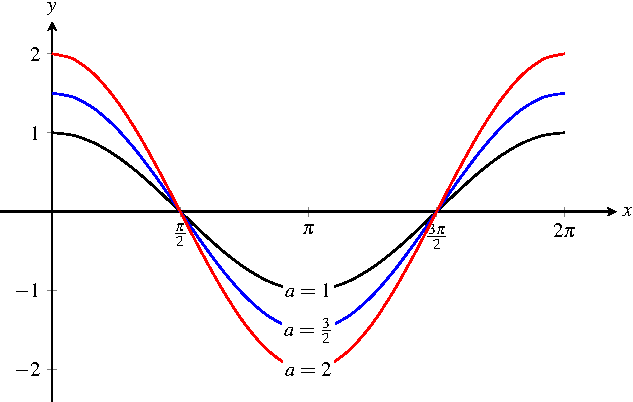
\includegraphics[scale=1.1]{image/13/cos-vertical-stretch.pdf}
\caption{%%
  Graphs of the function $f(x) = a \cos x$ for
  $a = \triple{1}{\frac{3}{2}}{2}$.
}
\label{fig:trigonometric:cos_vertical_stretch}
\end{figure}

\begin{figure}[!htbp]
\centering
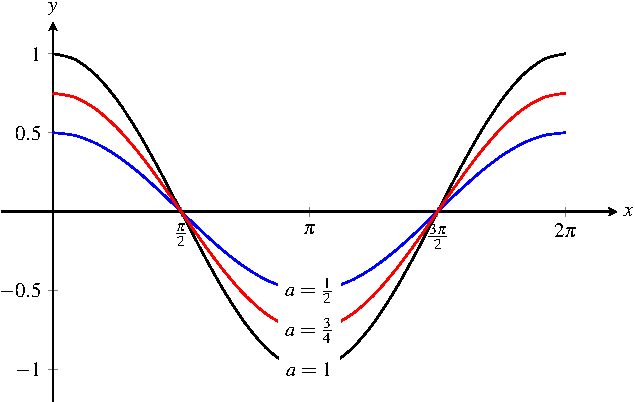
\includegraphics[scale=1.1]{image/13/cos-vertical-compress.pdf}
\caption{%%
  Graphs of the function $f(x) = a \cos x$ for
  $a = \triple{1}{\frac{1}{2}}{\frac{3}{4}}$.
}
\label{fig:trigonometric:cos_vertical_compress}
\end{figure}

\end{solution}
}{}


%%%%%%%%%%%%%%%%%%%%%%%%%%%%%%%%%%%%%%%%%%%%%%%%%%%%%%%%%%%%%%%%%%%%%%%%%%%

\section{Period and frequency}

Let $\triple{a}{b}{c}$ be real constants such that $a \neq 0$ and
$c \neq 0$ and let $x$ be a real variable.  Consider the sine and
cosine functions of the form
\[
f(x)
=
a \sin(cx) + b
%%
\qquad
\text{and}
\qquad
%%
g(x)
=
a \cos(cx) + b.
\]
You already know that the amplitude is the absolute value
$\absoluteValue{a}$ and the midline is $y = b$.  What effect does the
value of $c$ have on the graph of $f(x)$ and $g(x)$?  To understand
how the value of $c$ affects the graph of the sine and cosine
functions, consider the simpler functions $F(x) = \sin(cx)$ and
$G(x) = \cos(cx)$.
\Figure{subfig:trigonometric:sine_horizontal_stretch} shows graphs of
$F(x)$ for $c = \triple{1}{\frac{3}{4}}{\frac{1}{2}}$ and
\Figure{subfig:trigonometric:sine_horizontal_compress} shows some
graphs of $F(x)$ for $c = \triple{1}{\frac{3}{2}}{2}$.  The figures
show that when $0 < c < 1$ the value of $c$ stretches the graph of the
sine function along the horizontal direction.  However, when $c > 1$
the value of $c$ horizontally compresses the graph of the sine
function.  Thus the value of $c > 0$ has the effect of stretching or
compressing along the horizontal axis the graph of the sine function.

\begin{figure}[!htbp]
\centering
\subfigure[]{
  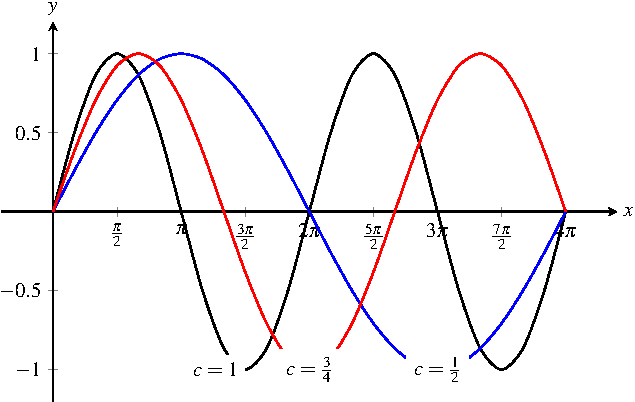
\includegraphics[scale=1.1]{image/13/sin-horizontal-stretch.pdf}
  \label{subfig:trigonometric:sine_horizontal_stretch}
}
%%
%%
\subfigure[]{
  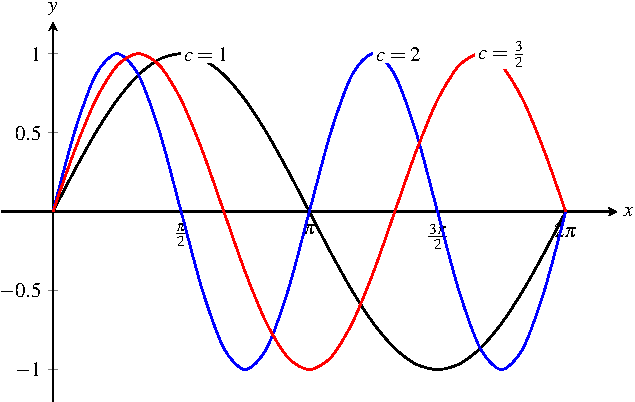
\includegraphics[scale=1.1]{image/13/sin-horizontal-compress.pdf}
  \label{subfig:trigonometric:sine_horizontal_compress}
}
\caption{%%
  Various graphs of the sine function $F(x) = \sin(cx)$ for
  (a)~$c = \triple{1}{\frac{3}{4}}{\frac{1}{2}}$ and
  (b)~$c = \triple{1}{\frac{3}{2}}{2}$.
}
\label{fig:trigonometric:sine_horizontal_stretch_compress}
\end{figure}

\begin{exercise}
Graph the cosine function $G(x) = \cos(cx)$ for
$c = \triple{1}{\frac{3}{4}}{\frac{1}{2}}$.  Also graph $G(x)$ for
$c = \triple{1}{\frac{4}{3}}{2}$.  If $c > 0$, describe the effect of
the value of $c$ on the graph of the cosine function.
\end{exercise}

\ifbool{showSolution}{
\begin{solution}
\Figures{subfig:trigonometric:cosine_horizontal_stretch}{subfig:trigonometric:cosine_horizontal_compress}
show various graphs of the cosine function $G(x) = \cos(cx)$ for
$c = \triple{1}{\frac{3}{4}}{\frac{1}{2}}$ and
$c = \triple{1}{\frac{4}{3}}{2}$.  As can be seen from the figures,
when $0 < c < 1$ the value of $c$ effectively stretches along the
horizontal direction the graph of the cosine function.  However, when
$c > 1$ the value of $c$ compresses along the horizontal direction the
graph of the cosine function.  In effect, the value of $c > 0$
stretches or compresses the graph of the cosine function along the
horizontal axis.

\begin{figure}[!htbp]
\centering
\subfigure[]{
  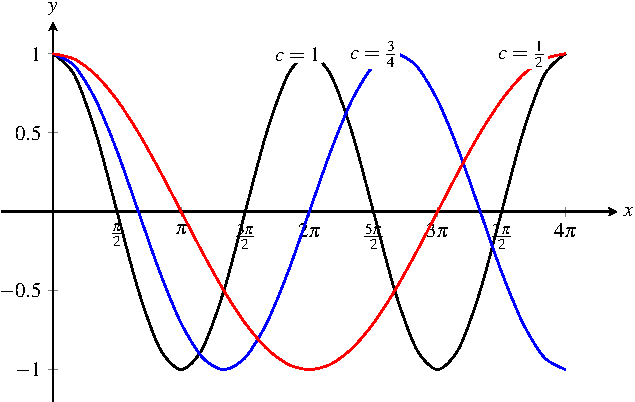
\includegraphics[scale=1.1]{image/13/cos-horizontal-stretch.pdf}
  \label{subfig:trigonometric:cosine_horizontal_stretch}
}
%%
%%
\subfigure[]{
  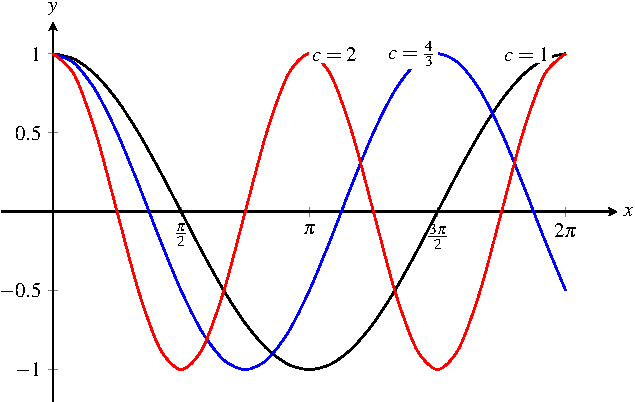
\includegraphics[scale=1.1]{image/13/cos-horizontal-compress.pdf}
  \label{subfig:trigonometric:cosine_horizontal_compress}
}
\caption{%%
  Various graphs of the cosine function $G(x) = \cos(cx)$ for
  (a)~$c = \triple{1}{\frac{3}{4}}{\frac{1}{2}}$ and
  (b)~$c = \triple{1}{\frac{4}{3}}{2}$.
}
\label{fig:trigonometric:cosine_horizontal_stretch_compress}
\end{figure}

\end{solution}
}{}

\begin{figure}[!htbp]
\centering
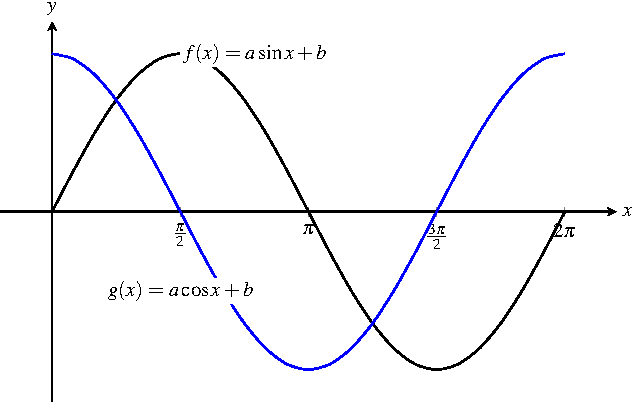
\includegraphics[scale=1.1]{image/13/sin-cos-cycle-default.pdf}
\caption{%%
  The functions $f(x) = a \sin x + b$ and $g(x) = a \cos x + b$ each
  requires $2\pi$ units of time to complete one cycle.
}
\label{fig:trigonometric:sine_cosine_one_cycle}
\end{figure}

The effect of the factor $c$ can also be understood in terms of the
amount of time required for the graph of a sine or cosine function to
complete one cycle.  Let $a \neq 0$ and $b$ be fixed real numbers and
suppose that $x$ is a real variable.
\Figure{fig:trigonometric:sine_cosine_one_cycle} shows graphs of the
functions $f(x) = a \sin x + b$ and $g(x) = a \cos x + b$.  If you
interpret the variable $x$ as representing time, then
\Figure{fig:trigonometric:sine_cosine_one_cycle} shows that the graph
of each of the functions $f(x)$ and $g(x)$ requires $2\pi$ units of
time to complete one cycle.  Now suppose that $c > 0$ is a fixed real
number and consider the functions $F(x) = a \sin(cx) + b$ and
$G(x) = a \cos(cx) + b$.  The effect of the factor $c$ is to change
the amount of time required for the graph of a sine or cosine function
to complete one cycle.  In many applications of trigonometric
functions, the amount of time required for the graph of a sine or
cosine function to complete one cycle is also called the
\emph{wavelength}.\footnote{
  See the video at
  \url{https://youtu.be/E-SPpUhzYZY}.
}

\begin{figure}[!htbp]
\centering
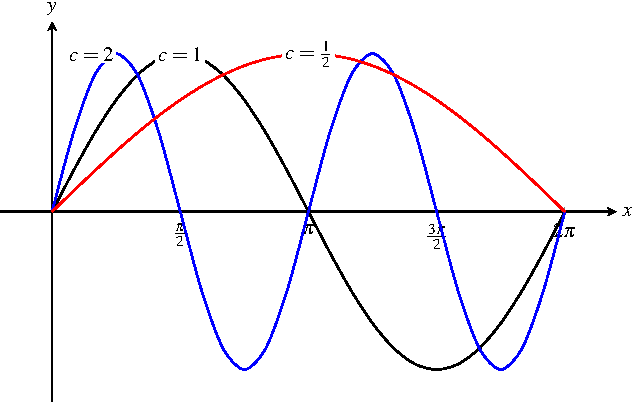
\includegraphics[scale=1.1]{image/13/sin-cycle.pdf}
\caption{%%
  Graphs of the sine function $F(x) = a \sin(cx) + b$ for
  $c = \triple{\frac{1}{2}}{1}{2}$.
}
\label{fig:trigonometric:sine_cycle}
\end{figure}

For example, \Figure{fig:trigonometric:sine_cycle} shows various
graphs of $F(x)$ for $c = \triple{\frac{1}{2}}{1}{2}$.  When $c = 1$
you have $F_1(x) = f(x) = a \sin x + b$, the graph of which requires
$2\pi$ units of time to complete one cycle.  When $c = 2$ you have
$F_2(x) = a \sin(2x) + b$, whose graph requires $\pi$ units of time to
complete one cycle.  Finally, when $c = \frac{1}{2}$ you have
$F_3(x) = a \sin(\frac{x}{2}) + b$, whose graph requires $4\pi$ units
of time to complete one cycle.  As can be seen from
\Figure{fig:trigonometric:sine_cycle}, when $0 < c < 1$ the graph of
$F(x)$ requires more time than the graph of $f(x)$ to complete one
cycle, which is due to the fact that $c$ horizontally stretches the
graph of the sine function.  However, when $c > 1$ the graph of $F(x)$
requires less time than the graph of $f(x)$ to complete one cycle, the
reason being that $c$ horizontally compresses the graph of the sine
function.  In other words, the value of $c > 0$ not only stretches or
compresses the graph of a sine function along the horizontal axis, the
number also shortens or lengthens the amount of time required for the
graph of a sine function to complete one cycle.
\Definition{def:trigonometric:sine_cosine_period} captures the idea of
the amount of time required for the graph of a sine or cosine function
to complete one cycle.

\begin{definition}
\label{def:trigonometric:sine_cosine_period}
\textbf{Period.}
Let $\triple{a}{b}{c}$ be real constants such that $a \neq 0$ and
$c \neq 0$.  Let $x$ be a real variable and consider the functions
\[
f(x)
=
a \sin(cx) + b
%%
\qquad
\text{and}
\qquad
%%
g(x)
=
a \cos(cx) + b.
\]
The amount of time required for the graphs of $f(x)$ and $g(x)$ to
complete one cycle is called the \emph{period} of the functions.  The
period of $f(x)$ and $g(x)$ is defined as $2\pi / \absoluteValue{c}$.
\end{definition}

\begin{exercise}
Calculate the period of $f(x) = \sin(3x)$.
\end{exercise}

\ifbool{showSolution}{
\begin{solution}
In the function $f(x) = \sin(3x)$, your $c$ value is $c = 3$.  Then
$f(x)$ has a period of $2\pi / 3$.
\end{solution}
}{}

\begin{exercise}
Consider the function $f(x) = \cos(cx)$.  Graph the function for
$c = \triple{\frac{1}{2}}{1}{\frac{4}{3}}$, where
$0 \leq x \leq 2\pi$.  When $c = 1$, how long does the graph of $f(x)$
take to complete one cycle?  Determine the period of $f(x)$ when
$c = \frac{4}{3}$.
\end{exercise}

\ifbool{showSolution}{
\begin{solution}
See \Figure{fig:trigonometric:cosine_cycle}.  When $c = 1$, the graph
of $f(x)$ requires $2\pi$ units of time to complete one cycle.  When
$c = \frac{4}{3}$, the period of $f(x)$ is
%%
\begin{align*}
\frac{2\pi}{4/3}
&=
2\pi \div \frac{4}{3} \\[4pt]
&=
2\pi \times \frac{3}{4} \\[4pt]
&=
\frac{3\pi}{2}.
\end{align*}
%%
In other words, when $c = \frac{4}{3}$ the graph of $f(x)$ requires
$\frac{3\pi}{2}$ units of time to complete one cycle.

\begin{figure}[!htbp]
\centering
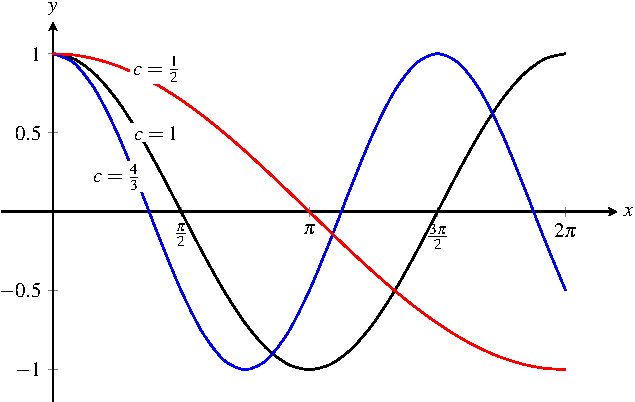
\includegraphics[scale=1.1]{image/13/cos-cycle.pdf}
\caption{%%
  Graphs of the function $f(x) = \cos(cx)$ for
  $c = \triple{\frac{1}{2}}{1}{\frac{4}{3}}$.
}
\label{fig:trigonometric:cosine_cycle}
\end{figure}

\end{solution}
}{}

\begin{exercise}
Let $c > 0$ be a fixed real number and consider the functions
$f(x) = \sin(cx)$ and $g(x) = \cos(-cx)$.  Prove that $f(x)$ and
$g(x)$ have the same period.
\end{exercise}

\ifbool{showSolution}{
\begin{solution}
The period of $f(x)$ is $2\pi / \absoluteValue{c}$, which simplifies
to $2\pi / c$ because $c$ is assumed to be positive.  The period of
$g(x)$ is $2\pi / \absoluteValue{-c}$.  Since $c$ is positive, then
$-c$ is negative and you have $\absoluteValue{-c} = c$.  Thus the
period of $g(x)$ is $2\pi / \absoluteValue{-c} = 2\pi / c$, which is
the same as the period of $f(x)$.
\end{solution}
}{}

\begin{exercise}
Let $\triple{a}{b}{c}$ be real constants such that $a \neq 0$ and
consider the function $f(x) = a \sin(cx) + b$.  Determine all values
of $c$ such that the period of $f(x)$ is $\frac{\pi}{2}$.
\end{exercise}

\ifbool{showSolution}{
\begin{solution}
The period of $f(x)$ can be written as the equation
$\frac{2\pi}{\absoluteValue{c}} = \frac{\pi}{2}$.  Multiply both sides
by $\absoluteValue{c}$ to get
$2\pi = \frac{\pi}{2} \absoluteValue{c}$, which upon solving for
$\absoluteValue{c}$ results in
%%
\begin{align*}
\absoluteValue{c}
&=
\frac{2}{\pi} \times 2\pi \\[4pt]
&=
4.
\end{align*}
%%
This means that when $c = 4$ the function $f(x)$ has a period of
$\frac{\pi}{2}$ because
\[
\frac{2\pi}{\absoluteValue{4}}
=
\frac{2\pi}{4}
=
\frac{\pi}{2}.
\]
Furthermore, when $c = -4$ the function $f(x)$ also has a period of
$\frac{\pi}{2}$.  The reason is that
\[
\frac{2\pi}{\absoluteValue{-4}}
=
\frac{2\pi}{4}
=
\frac{\pi}{2}.
\]
Therefore when $c = \pm 4$ the function $f(x)$ has a period of
$\frac{\pi}{2}$.
\end{solution}
}{}

\begin{figure}[!htbp]
\centering
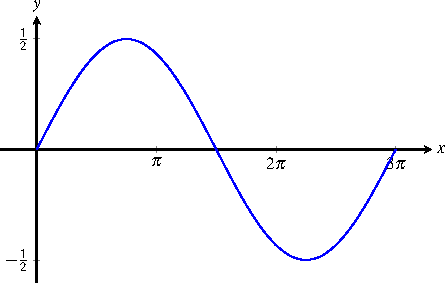
\includegraphics[scale=1.1]{image/13/half-sin-3pi.pdf}
\caption{%%
  A trigonometric function that has a period of $3\pi$.
}
\label{fig:trigonometric:half_sine_3pi}
\end{figure}

\begin{example}
Derive a formula for the function graphed in
\Figure{fig:trigonometric:half_sine_3pi}.
\end{example}

\begin{solution}
\Figure{fig:trigonometric:half_sine_3pi} shows a graph of a sine
function whose midline is $y = 0$, which means that the figure
possibly shows a function of the form $f(x) = a \sin(cx)$.  The
highest and lowest values of the function are $\frac{1}{2}$ and
$-\frac{1}{2}$, respectively, so that the amplitude is
$a = \frac{1}{2}$.  The graph of the function requires $3\pi$ units of
time to complete one cycle, thus the function has a period of $3\pi$.
The value of $c$ is related to the period by the equation
$2\pi / \absoluteValue{c} = 3\pi$.  Solve the latter equation for
$\absoluteValue{c}$ to get
\[
\absoluteValue{c}
=
\frac{2\pi}{3\pi}
=
\frac{2}{3}.
\]
You may assume that $c > 0$.  Therefore it is possible that
\Figure{fig:trigonometric:half_sine_3pi} shows a graph of the function
$f(x) = \frac{1}{2} \sin(\frac{2}{3} x)$.
\end{solution}

\begin{figure}[!htbp]
\centering
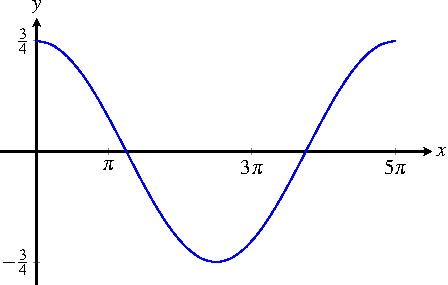
\includegraphics[scale=1.1]{image/13/3quarter-cos-5pi.pdf}
\caption{%%
  A trigonometric function whose period is $5\pi$.
}
\label{fig:trigonometric:3quarter_cos_5pi}
\end{figure}

\begin{exercise}
Determine a formula for the function graphed in
\Figure{fig:trigonometric:3quarter_cos_5pi}.
\end{exercise}

\ifbool{showSolution}{
\begin{solution}
\Figure{fig:trigonometric:3quarter_cos_5pi} possibly shows a graph of
a cosine function whose midline is $y = 0$.  Then the function shown
in the figure might be of the form $f(x) = a \cos(cx)$.  The highest
and lowest values of the function are $\frac{3}{4}$ and
$-\frac{3}{4}$, so that the amplitude is $a = \frac{3}{4}$.  If you
assume that $c > 0$, then the value of $c$ is related to the period by
the equation $\frac{2\pi}{c} = 5\pi$.  Solving the latter equation for
$c$ shows that
\[
c
=
\frac{2\pi}{5\pi}
=
\frac{2}{5}.
\]
Therefore the function whose graph is shown in
\Figure{fig:trigonometric:3quarter_cos_5pi} can be described by the
formula $f(x) = \frac{3}{4} \cos(\frac{2}{5} x)$.
\end{solution}
}{}

\begin{table}[!htbp]
\centering
\begin{tabular}{ccccccccccccc} \toprule
Month & Jan & Feb  & Mar  & Apr  & May  & Jun  & Jul  & Aug & Sep  & Oct  & Nov & Dec \\
Mean  & 26  & 25.8 & 23.9 & 20.3 & 16.7 & 14.1 & 13.5 & 15  & 17.3 & 19.7 & 22  & 24.2 \\\bottomrule
\end{tabular}

\caption{%%
  The mean maximum temperature~($\degreec{}$) of each month for the city of
  Melbourne, Victoria, Australia.  The mean was calculated using
  temperature data for the years from $1855$ to $2015$.  The mean
  temperatures are provided by the Bureau of Meteorology of
  Australia.
}
\label{tab:trigonometric:mean_maximum_temperature}
\end{table}

\begin{figure}[!htbp]
\centering
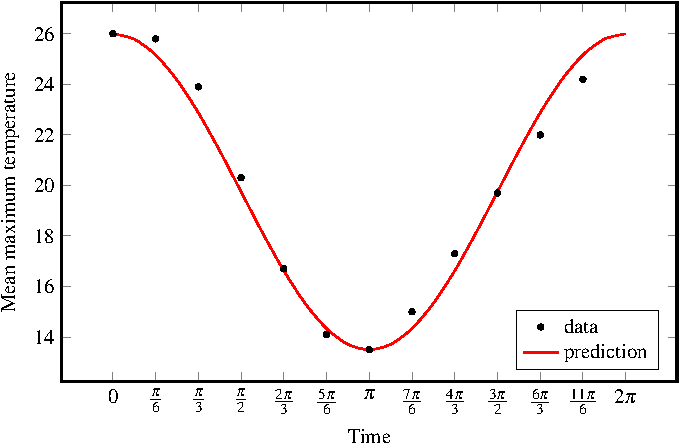
\includegraphics[scale=1.1]{image/13/mean-max-temperature.pdf}
\caption{%%
  The mean maximum temperature~($\degreec{}$) versus time of the year
  for the city of Melbourne, Victoria, Australia.  Each tick on the
  horizontal axis corresponds to a month of the year.  So $0$
  corresponds to January, $\frac{\pi}{6}$ corresponds to February,
  $\frac{\pi}{3}$ corresponds to March, and so on, up to
  $\frac{11\pi}{6}$ corresponding to December.  The black dots show
  the data from \Table{tab:trigonometric:mean_maximum_temperature}.
  The red curve is a graph of the prediction function as defined by
  \Equation{eqn:trigonometric:mean_max_temperature_prediction}.
}
\label{fig:trigonometric:mean_max_temperature}
\end{figure}

\begin{example}
\label{eg:trigonometric:mean_maximum_temperature}
\textbf{Mean maximum temperature.}
\Table{tab:trigonometric:mean_maximum_temperature} shows the mean
maximum temperature~($\degreec{}$) of each month for
Melbourne.\footnote{
  The data are taken from the website
  \url{http://web.archive.org/web/20180708014708/http://www.bom.gov.au/climate/averages/tables/cw_086071.shtml},
  accessed 2018-07-08.
}
%%
\begin{packedenum}
\item\label{subeg:trigonometric:mean_max_temperature_graph}
  Let the twelve months correspond to equally spaced numbers from $0$
  to $2\pi$.  Divide $2\pi$ by $12$ months to get
  $\delta = \frac{2\pi}{12} = \frac{\pi}{6}$.  Starting from $i = 0$,
  let $0 \times \delta = 0$ represent January, let
  $1 \times \delta = \delta$ represent February, let
  $2 \times \delta = 2\delta$ represent March, and so on, up to
  $11 \times \delta = 11\delta$ representing December.  Values of
  $i\delta$, for $i = \seq{0}{1}{11}$, can now be interpreted as time.
  Produce a graph of $i\delta$ versus the mean maximum temperature
  corresponding to $i\delta$.  Explain what you notice about your
  graph.

\item\label{subeg:trigonometric:mean_max_temperature_midline}
  Suppose that the data in
  \Table{tab:trigonometric:mean_maximum_temperature} can be modelled
  as a function of the form $f(x) = a \cos(cx) + b$, where $x$
  represents a time of the year and $f(x)$ represents the mean maximum
  temperature~($\degreec{}$) corresponding to $x$.  Use your graph and
  the data table to estimate the value of $b$.

\item\label{subeg:trigonometric:mean_max_temperature_amplitude}
  Estimate the value of the amplitude $a$.

\item\label{subeg:trigonometric:mean_max_temperature_c}
  Assume that the period of the function $f(x)$ is $2\pi$ and that
  $c > 0$.  Estimate the value of $c$.  Graph your function $f(x)$
  together with the graph
  from \Part{subeg:trigonometric:mean_max_temperature_graph}.

\item\label{subeg:trigonometric:mean_max_temperature_RMSE_R2}
  Calculate the root mean square error~(RMSE) and the coefficient of
  determination $R^2$ of the function $f(x)$.  Use the
  values of the RMSE and $R^2$ to explain how well the function $f(x)$
  models the given data.
\end{packedenum}
\end{example}

\begin{solution}
\solutionpart{subeg:trigonometric:mean_max_temperature_graph}
\Figure{fig:trigonometric:mean_max_temperature} shows a graph of the
data from \Table{tab:trigonometric:mean_maximum_temperature}.  The
dots in the figure seem to follow the graph of a cosine function.
This suggests that the mean maximum temperature~($\degreec{}$) can be
modelled as a function of the form $f(x) = a \cos(cx) + b$, where the
parameters $\triple{a}{b}{c}$ are to be estimated from the data.

\solutionpart{subeg:trigonometric:mean_max_temperature_midline}
The value $b$ of the midline of a cosine function is the mean of the
lowest and highest values of the function.  From
\Table{tab:trigonometric:mean_maximum_temperature} the lowest and
highest temperature values are $13.5$ and $26$, respectively.  The
mean of these two values is
\[
\frac{13.5 + 26}{2}
=
19.75
\]
so that the value of the midline of $f(x)$ can be estimated as
$b = 19.75$.

\solutionpart{subeg:trigonometric:mean_max_temperature_amplitude}
The amplitude of a cosine function is the absolute value of the
difference between the highest value of the function and the value of
the midline.
From \Part{subeg:trigonometric:mean_max_temperature_midline} you know
that the highest temperature value is $26$ and the value of the
midline is estimated to be $b = 19.75$.  Then the amplitude can be
estimated as
\[
a
=
\absoluteValue{26 - 19.75}
=
\absoluteValue{6.25}
=
6.25.
\]

\solutionpart{subeg:trigonometric:mean_max_temperature_c}
By definition, the period of the cosine function $f(x)$ can be written
as $\frac{2\pi}{\absoluteValue{c}} = 2\pi$.  Multiply both sides by
$\absoluteValue{c}$ to get $2\pi = 2\pi\absoluteValue{c}$.  Solve the
latter equation for $\absoluteValue{c}$ to see that
$\absoluteValue{c} = 1$.  Assuming that $c > 0$, the value of $c$ can
be estimated as $c = 1$.  Thus the mean maximum temperature can be
modelled as the function
%%
\begin{equation}
\label{eqn:trigonometric:mean_max_temperature_prediction}
f(x)
=
6.25 \cos(x) + 19.75
\end{equation}
%%
which is graphed in \Figure{fig:trigonometric:mean_max_temperature}.

\solutionpart{subeg:trigonometric:mean_max_temperature_RMSE_R2}
The root mean square error of $f(x)$ is approximately $0.606277$.  The
sum of squared errors is $\text{SSE} \approx 4.410863$ and the total
sum of squares is $\text{TSS} \approx 226.7225$.  The coefficient of
determination is
%%
\begin{align*}
R^2
&=
1 - \frac{\text{SSE}}{\text{TSS}} \\[4pt]
&\approx
0.9805.
\end{align*}
%%
The low value of the RMSE and the high value of $R^2$ suggest that the
function $f(x)$ models the given data pretty well.
\end{solution}

\begin{table}[!htbp]
\centering
\begin{tabular}{ccccccccccccc} \toprule
Month & Jan  & Feb  & Mar  & Apr  & May  & Jun & Jul & Aug & Sep  & Oct  & Nov  & Dec  \\
Mean  & 19.1 & 19.1 & 17.5 & 14.7 & 11.7 & 9.4 & 8.7 & 10  & 12.3 & 14.7 & 16.1 & 17.7 \\\bottomrule
\end{tabular}

\caption{%%
  The mean temperature~($\degreec{}$) at $9$~am of each month for the
  city of Melbourne, Victoria, Australia.  The mean was calculated
  using temperature data for the years from $1955$ to $2010$.  The
  mean temperatures are provided by the Bureau of Meteorology of
  Australia.
}
\label{tab:trigonometric:mean_9am_temperature}
\end{table}

\begin{exercise}
\textbf{Mean $9$~am temperature.}
\Table{tab:trigonometric:mean_9am_temperature} shows the mean
temperature~($\degreec{}$) at $9$~am of each month for
Melbourne.\footnote{
  The data are available at
  \url{http://web.archive.org/web/20180710193217/http://www.bom.gov.au/climate/averages/tables/cw_086071.shtml},
  accessed 2018-07-10.
}
%%
\begin{packedenum}
\item\label{subex:trigonometric:mean_9am_temperature_graph}
  As in \Part{subeg:trigonometric:mean_max_temperature_graph} of
  \Example{eg:trigonometric:mean_maximum_temperature}, associate the
  months with equally spaced numbers from $0$ to $2\pi$.  Produce a
  scatter plot of the data in
  \Table{tab:trigonometric:mean_9am_temperature}, where the horizontal
  axis represents a time of the year and the vertical axis represents
  the mean temperature~($\degreec{}$) at $9$~am.  Explain what you
  notice about the graph.

\item\label{subex:trigonometric:mean_9am_temperature_model}
  Suppose that the data in
  \Table{tab:trigonometric:mean_9am_temperature} can be modelled as a
  function of the form $f(x) = a \cos(cx) + b$, where $x$ represents a
  time of the year and $f(x)$ represents the mean $9$~am
  temperature~($\degreec{}$) corresponding to $x$.  Use the given data
  to estimate the values of the parameters $\triple{a}{b}{c}$.  You
  may assume that the period of $f(x)$ is $2\pi$ and that $c > 0$.
  Graph the function $f(x)$ together with the scatter plot
  from \Part{subex:trigonometric:mean_9am_temperature_graph}.

\item\label{subex:trigonometric:mean_9am_temperature_assess}
  Calculate the root mean square error~(RMSE) and the coefficient of
  determination $R^2$ of $f(x)$.  Use the values of the RMSE and $R^2$
  to help you decide how well the function $f(x)$ models the data in
  \Table{tab:trigonometric:mean_9am_temperature}.
\end{packedenum}
\end{exercise}

\ifbool{showSolution}{
\begin{solution}
\solutionpart{subex:trigonometric:mean_9am_temperature_graph}
\Figure{fig:trigonometric:mean_9am_temperature} shows a scatter plot
of the data in \Table{tab:trigonometric:mean_9am_temperature}.  As can
be seen from the figure, the black dots seem to follow the graph of a
cosine function.  This suggests that the given data can be modelled as
a function of the form $f(x) = a \cos(cx) + b$, where the parameters
$\triple{a}{b}{c}$ are to be estimated from the data.

\begin{figure}[!htbp]
\centering
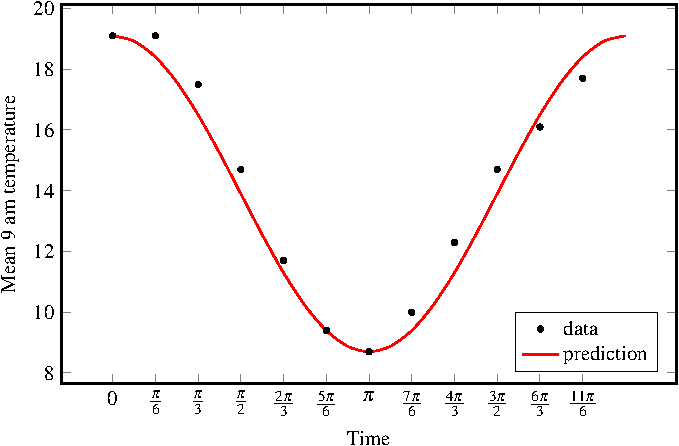
\includegraphics[scale=1.1]{image/13/mean-9am-temperature.pdf}
\caption{%%
  The mean temperature~($\degreec{}$) at $9$~am for each time of the
  year for the city of Melbourne, Victoria, Australia.  Each tick on
  the horizontal axis corresponds to a month of the year.  So $0$
  corresponds to January, $\frac{\pi}{6}$ corresponds to February, and
  so on.  The black dots show the data in
  \Table{tab:trigonometric:mean_9am_temperature}.  The red curve is a
  graph of the prediction function as defined by
  \Equation{eqn:trigonometric:mean_9am_temperature}.
}
\label{fig:trigonometric:mean_9am_temperature}
\end{figure}

\solutionpart{subex:trigonometric:mean_9am_temperature_model}
Suppose that the data in
\Table{tab:trigonometric:mean_9am_temperature} can be modelled as a
function of the form $f(x) = a \cos(cx) + b$, where $x$ represents a
time of the year and $f(x)$ represents the mean $9$~am
temperature~($\degreec{}$) corresponding to $x$.  The value $b$ of the
midline is the average of the lowest and highest values in the table.
The minimum and maximum values in the table are $8.7$ and $19.1$,
respectively, so
\[
b
=
\frac{8.7 + 19.1}{2}
=
13.9.
\]
The value of the amplitude $a$ is the absolute value of the difference
between the highest value in the table and the value of the midline.
So you have
\[
a
=
\absoluteValue{19.1 - 13.9}
=
\absoluteValue{5.2}
=
5.2.
\]
The period of $f(x)$ can be written as the equation
$\frac{2\pi}{\absoluteValue{c}} = 2\pi$, which can be solved for
$\absoluteValue{c}$ to obtain $\absoluteValue{c} = 1$.  As you have
assumed that $c > 0$, it follows that $c = 1$.  Therefore the function
$f(x)$ can be written as
%%
\begin{equation}
\label{eqn:trigonometric:mean_9am_temperature}
f(x)
=
5.2 \cos x + 13.9
\end{equation}
%%
which is graphed in \Figure{fig:trigonometric:mean_9am_temperature}.

\solutionpart{subex:trigonometric:mean_9am_temperature_assess}
The root mean square error of $f(x)$ is
$\text{RMSE} \approx 0.641875$.  The sum of squared errors is
$\text{SSE} \approx 4.944043$, the total sum of squares is
$\text{TSS} = 156.03$, so the coefficient of determination of $f(x)$
is
\[
R^2
=
1 - \frac{\text{SSE}}{\text{TSS}}
\approx
0.968314.
\]
The low value of the RMSE and the high value of $R^2$ suggest that the
function $f(x)$ models the data in
\Table{tab:trigonometric:mean_9am_temperature} very well.
\end{solution}
}{}

The \emph{frequency} of a sine or cosine function is a concept that is
closely related to the period.  The frequency counts the number of
cycles per unit time.  For example, if the graph of a sine function
$f(x)$ requires one second to complete one cycle, you would say that
the frequency of the function is one cycle per second.  In various
applications of the sine and cosine functions, the number of cycles
per second is usually expressed in terms of \emph{hertz} and written
as Hz.  In the above example, you would say that the function $f(x)$
has a frequency of $1$~Hz.  As another example, suppose that the graph
of a cosine function $g(x)$ completes one cycle in $0.5$ seconds.
Then in one second the graph of $g(x)$ would complete two cycles and
hence you would say that the frequency of $g(x)$ is $2$~Hz.
\Definition{def:trigonometric:sine_cosine_frequency} provides a way to
calculate the frequencies of sine and cosine functions.

\begin{definition}
\label{def:trigonometric:sine_cosine_frequency}
\textbf{Frequency.}
Let $\triple{a}{b}{c}$ be real constants such that $a \neq 0$ and
$c \neq 0$ and let $x$ be a real variable.  Consider the functions
\[
f(x)
=
a \sin(cx) + b
%%
\qquad
\text{and}
\qquad
%%
g(x)
=
a \cos(cx) + b
\]
each of which has a period of $p = 2 \pi / \absoluteValue{c}$.  The
\emph{frequency} of $f(x)$ and $g(x)$ is the number
%%
\begin{equation}
\label{eqn:trigonometric:frequency_sin_cos}
\frac{1}{p}
=
\frac{\absoluteValue{c}}{2\pi}.
\end{equation}
\end{definition}

\begin{exercise}
Read about hertz and Heinrich Hertz at the following websites:
%%
\begin{packeditem}
\item \url{https://en.wikipedia.org/wiki/Hertz}

\item \url{https://en.wikipedia.org/wiki/Heinrich_Hertz}
\end{packeditem}
\end{exercise}

\begin{example}
Let $c \neq 0$ be a real constant and consider the function
$f(x) = \cos(cx)$.  Suppose that the graph of $f(x)$ completes one
cycle in $0.25$ seconds.
%%
\begin{packedenum}
\item\label{subeg:trigonometric:cos_1_cycle_0.25_seconds_period}
  Determine the period and frequency of $f(x)$.

\item\label{subeg:trigonometric:cos_1_cycle_0.25_seconds_c_factor}
  Calculate the possible values for $c$.
\end{packedenum}
\end{example}

\begin{solution}
\solutionpart{subeg:trigonometric:cos_1_cycle_0.25_seconds_period}
The period of $f(x)$ is the amount of time required for the graph of
$f(x)$ to complete one cycle.  Since it is assumed that the graph of
$f(x)$ completes one cycle in $0.25 = 1/4$ seconds, then $f(x)$ has a
period of $p = 1/4$ seconds.  The frequency of $f(x)$ is
%%
\begin{align*}
\frac{1}{p}
&=
1 \div \frac{1}{4} \\[4pt]
&=
1 \times \frac{4}{1} \\[4pt]
&=
4
\end{align*}
%%
cycles per second or $4$~Hz.

\solutionpart{subeg:trigonometric:cos_1_cycle_0.25_seconds_c_factor}
Let $p$ be the period of $f(x)$ so that the frequency of $f(x)$ is
$1 / p$.  From \Equation{eqn:trigonometric:frequency_sin_cos}, you
know that the frequency of $f(x)$ is related to the value
$\absoluteValue{c}$ as follows:
\[
\frac{1}{p}
=
\frac{\absoluteValue{c}}{2\pi}.
\]
From \Part{subeg:trigonometric:cos_1_cycle_0.25_seconds_period} you
know that $f(x)$ has a frequency of $4$~Hz, which can be used to
simplify the latter equation to $4 = \frac{\absoluteValue{c}}{2\pi}$.
Solve the last equation for $\absoluteValue{c}$ to get
$\absoluteValue{c} = 4 \times 2\pi = 8\pi$.  If $c = 8\pi$ then you
would get $\absoluteValue{c} = \absoluteValue{8\pi} = 8\pi$.
Furthermore, if $c = -8\pi$ then you would have
$\absoluteValue{c} = \absoluteValue{-8\pi} = 8\pi$.  Therefore the
possible values for $c$ are $c = \pm 8\pi$.
\end{solution}

\begin{exercise}
Consider the function $f(x) = \sin \frac{x}{2}$.
%%
\begin{packedenum}
\item\label{subeg:trigonometric:sin_half_period}
  Calculate the period of $f(x)$.

\item\label{subeg:trigonometric:sin_half_frequency}
  Use the period to determine the frequency of $f(x)$.
\end{packedenum}
\end{exercise}

\ifbool{showSolution}{
\begin{solution}
\solutionpart{subeg:trigonometric:sin_half_period}
Your $c$ value is $c = \frac{1}{2}$ and so the required period is
%%
\begin{align*}
\frac{2\pi}{1/2}
&=
2\pi \div \frac{1}{2} \\[4pt]
&=
2\pi \times 2 \\[4pt]
&=
4\pi.
\end{align*}

\solutionpart{subeg:trigonometric:sin_half_frequency}
Since the period is $p = 4\pi$, then the frequency is
$1/p = \frac{1}{4\pi}$.
\end{solution}
}{}

\begin{exercise}
A trigonometric function $f(x)$ has an amplitude of $3$, a midline of
$y = 4$, and a period of $\frac{4\pi}{3}$.  Determine two possible
formulae for $f(x)$.  Calculate the frequency of $f(x)$.
\end{exercise}

\ifbool{showSolution}{
\begin{solution}
You are given an amplitude of $\absoluteValue{a} = 3$ and the midline
value $b = 4$.  If $c$ is a real constant, then $f(x)$ is possibly a
sine function that can be written as $f(x) = \pm 3 \sin(cx) + 4$ or a
cosine function of the form $f(x) = \pm 3 \cos(cx) + 4$.  The
remaining problem is to determine a value for $c$.

The period is related to the value of $c$ via the equation
$\frac{2\pi}{\absoluteValue{c}} = \frac{4\pi}{3}$.  Multiply both
sides by $\absoluteValue{c}$ and simplify to get
$2\pi = \frac{4\pi}{3} \absoluteValue{c}$.  To solve for
$\absoluteValue{c}$, first multiply both sides by $3$, then divide
both sides by $4\pi$, and finally simplify to obtain
%%
\begin{align*}
\absoluteValue{c}
&=
\frac{3}{4\pi} \times 2\pi \\[4pt]
&=
\frac{3 \times 2\pi}{4\pi} \\[4pt]
&=
\frac{3}{2}.
\end{align*}
%%
The possible values for $c$ are $c = \pm \frac{3}{2}$.  If you assume
that $c > 0$, then you have $c = \frac{3}{2}$ so that $f(x)$ is
possibly the sine function $f(x) = \pm 3 \sin(\frac{3}{2}x) + 4$ or
the cosine function $f(x) = \pm 3 \cos(\frac{3}{2}x) + 4$.

If $p$ is the period of $f(x)$, then the frequency of $f(x)$ is
defined as the number $1 / p$.  Since $f(x)$ has a period of
$p = \frac{4\pi}{3}$, then $f(x)$ has a frequency of
%%
\begin{align*}
\frac{1}{p}
&=
\frac{1}{4\pi/3} \\[4pt]
&=
1 \times \frac{3}{4\pi} \\[4pt]
&=
\frac{3}{4\pi}.
\end{align*}
\end{solution}
}{}

\begin{figure}[!htbp]
\centering
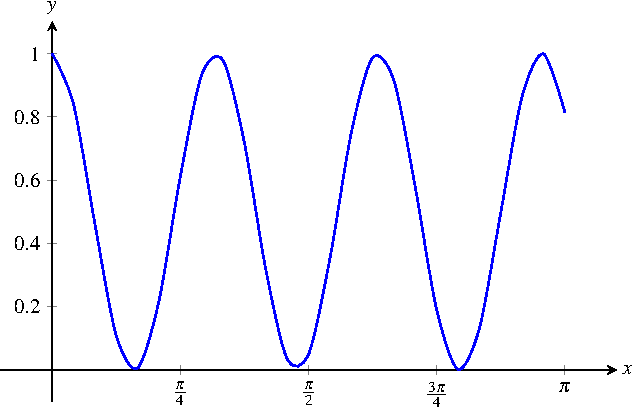
\includegraphics[scale=1.1]{image/13/blinking-light.pdf}
\caption{%%
  A graph of a function that models the behaviour of a blinking light
  bulb.
}
\label{fig:trigonometric:blinking_light}
\end{figure}

\begin{example}
\textbf{Blinking light.}
A light bulb is switched on and alternates between on and off.  Thus
the light bulb goes on, off, on, off, on, off, etc.  The light bulb is
on for a brief moment, then goes off for one second, and is on again.
The cycle repeats for as long as electricity is connected to the light
bulb.  Use a trigonometric function to model the blinking light bulb.
Produce a graph of your function from zero up to $\pi$ seconds.
\end{example}

\begin{solution}
Suppose that $1$~(one) means that the light bulb is on and $0$~(zero)
means that the light bulb is off.  The behaviour of the blinking light
bulb can be described as a sequence of $1$ and $0$:
\[
\seqi{\pair{1}{0}}{\pair{1}{0}}{\pair{1}{0}}
\]
The sequence can be modelled as a function of the form
$f(x) = a \cos(cx) + b$.  The highest and lowest values of $f(x)$ are
$1$ and $0$, respectively.  The average of these two extreme values is
the value of the midline.  That is, the value of $b$ is
\[
b
=
\frac{1 + 0}{2}
=
\frac{1}{2}.
\]
The amplitude is the difference between the highest value and the
value of the midline, hence
$a = 1 - \frac{1}{2} = \frac{1}{2}$.  The time between two consecutive
on is one second so the period is one second.  Using the definition of
the period, you have
$\frac{2\pi}{\absoluteValue{c}} = 1$.  Solve the latter equation for
$\absoluteValue{c}$ to get $\absoluteValue{c} = 2\pi$.  Assuming that
$c$ is positive, then you have $c = 2\pi$.  Conclude that the blinking
light bulb can be modelled as the function
$f(x) = \frac{1}{2} \cos(2\pi x) + \frac{1}{2}$, which is graphed in
\Figure{fig:trigonometric:blinking_light}.
\end{solution}


%%%%%%%%%%%%%%%%%%%%%%%%%%%%%%%%%%%%%%%%%%%%%%%%%%%%%%%%%%%%%%%%%%%%%%%%%%%

\section{Horizontal shift}

In this section, you will investigate another property of the graphs
of sine and cosine functions.  Up to this point, you have learnt about
how to stretch the graph of a sine or cosine function along the
horizontal and vertical axes.  You have also learnt about how to
vertically shift the graph of a sine or cosine function.  What remains
to be discussed is how to shift the graph of a sine or cosine function
along the horizontal axis.

\begin{figure}[!htbp]
\centering
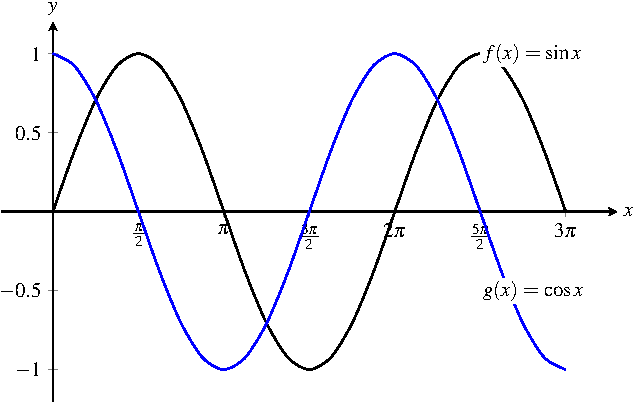
\includegraphics[scale=1.1]{image/13/sin-cos.pdf}
\caption{%%
  Graphs of the trigonometric functions $f(x) = \sin x$ and
  $g(x) = \cos x$ from $x = 0$ to $x = 3\pi$.
}
\label{fig:trigonometric:standard_sine_cosine}
\end{figure}

What does it mean to horizontally shift the graph of a trigonometric
function?  To answer this question, consider
\Figure{fig:trigonometric:standard_sine_cosine} which shows graphs of
the functions $f(x) = \sin x$ and $g(x) = \cos x$.  Note that you can
obtain the graph of the cosine function $g(x)$ by shifting the graph
of the sine function $f(x)$ to the left.  Looking at the graphs in
\Figure{fig:trigonometric:standard_sine_cosine}, the required amount
of horizontal shift is approximately $\frac{\pi}{2}$ units to the
left.  Thus it is reasonable to assume that the cosine function $g(x)$
can be written in terms of the sine function as
$h(x) = \sin(x + \frac{\pi}{2})$ and therefore you might conclude that
$\cos x = \sin(x + \frac{\pi}{2})$.

\begin{exercise}
You will verify that the equation $\cos x = \sin(x + \frac{\pi}{2})$
is true, especially for some special values of $x$.
%%
\begin{packedenum}
\item\label{subex:trigonometric:sin_left_shift_0}
  Let $x = 0$.  Calculate the exact values of $\cos x$ and
  $\sin(x + \frac{\pi}{2})$.

\item\label{subex:trigonometric:sin_left_shift_pi_half}
  Let $x = \frac{\pi}{2}$.  Calculate the exact values of $\cos x$ and
  $\sin(x + \frac{\pi}{2})$.

\item\label{subex:trigonometric:sin_left_shift_pi}
  Let $x = \pi$.  Calculate the exact values of $\cos x$ and
  $\sin(x + \frac{\pi}{2})$.

\item\label{subex:trigonometric:sin_left_shift_3pi_half}
  Let $x = \frac{3\pi}{2}$.  Calculate the exact values of $\cos x$
  and $\sin(x + \frac{\pi}{2})$.
\end{packedenum}
\end{exercise}

\ifbool{showSolution}{
\begin{solution}
\solutionpart{subex:trigonometric:sin_left_shift_0}
If $x = 0$, then $\sin(0 + \frac{\pi}{2}) = \sin\frac{\pi}{2} = 1$.
You also know that $\cos 0 = 1$.

\solutionpart{subex:trigonometric:sin_left_shift_pi_half}
If $x = \frac{\pi}{2}$, then
$\sin(\frac{\pi}{2} + \frac{\pi}{2}) = \sin \pi = 0$.  Furthermore,
you have $\cos \frac{\pi}{2} = 0$.

\solutionpart{subex:trigonometric:sin_left_shift_pi}
If $x = \pi$, then
$\sin(\pi + \frac{\pi}{2}) = \sin \frac{3\pi}{2} = -1$.  You also have
$\cos \pi = -1$.

\solutionpart{subex:trigonometric:sin_left_shift_3pi_half}
If $x = \frac{3\pi}{2}$, then
$\sin(\frac{3\pi}{2} + \frac{\pi}{2}) = \sin 2\pi = 0$.  You also have
$\cos \frac{3\pi}{2} = 0$.
\end{solution}
}{}

\Figure{fig:trigonometric:standard_sine_cosine} shows that you can
also obtain the graph of the function $f(x) = \sin x$ in terms of the
function $g(x) = \cos x$.  To do so, you can shift the graph of the
cosine function $g(x)$ along the horizontal axis.  The amount of
horizontal shift is approximately $\frac{\pi}{2}$ units to the right.
In other words, it is reasonable to assume that the sine function
$f(x)$ can be written in terms of the cosine function as
$h(x) = \cos(x - \frac{\pi}{2})$.  Therefore you might conclude that
$\sin x = \cos(x - \frac{\pi}{2})$.
\Definition{def:trigonometric:horizontal_shift} summarised the idea of
the horizontal shift of the graph of a trigonometric function.

\begin{exercise}
You will verify that the equation $\sin x = \cos(x - \frac{\pi}{2})$
is true, especially for certain special values of $x$.
%%
\begin{packedenum}
\item\label{subex:trigonometric:cos_right_shift_0}
  If $x = 0$, calculate the exact values of $\sin x$ and
  $\cos(x - \frac{\pi}{2})$.

\item\label{subex:trigonometric:cos_right_shift_pi_half}
  If $x = \frac{\pi}{2}$, calculate the exact values of $\sin x$ and
  $\cos(x - \frac{\pi}{2})$.

\item\label{subex:trigonometric:cos_right_shift_pi}
  If $x = \pi$, calculate the exact values of $\sin x$ and
  $\cos(x - \frac{\pi}{2})$.

\item\label{subex:trigonometric:cos_right_shift_3pi_half}
  If $x = \frac{3\pi}{2}$, calculate the exact values of $\sin x$ and
  $\cos(x - \frac{\pi}{2})$.
\end{packedenum}
\end{exercise}

\ifbool{showSolution}{
\begin{solution}
\solutionpart{subex:trigonometric:cos_right_shift_0}
If $x = 0$, then $\sin 0 = 0$.  Note that
$0 - \frac{\pi}{2} = -\frac{\pi}{2}$ radians is equivalent to
$\frac{3\pi}{2}$ radians.  Then
$\cos(0 - \frac{\pi}{2}) = \cos \frac{3\pi}{2} = 0$.

\solutionpart{subex:trigonometric:cos_right_shift_pi_half}
If $x = \frac{\pi}{2}$, then $\sin \frac{\pi}{2} = 1$.  Note that you
have $\frac{\pi}{2} - \frac{\pi}{2} = 0$.  Then you have
$\cos(\frac{\pi}{2} - \frac{\pi}{2}) = \cos 0 = 1$.

\solutionpart{subex:trigonometric:cos_right_shift_pi}
If $x = \pi$, then $\sin \pi = 0$.  Note that
$\pi - \frac{\pi}{2} = \frac{\pi}{2}$, which can be used to write
$\cos(\pi - \frac{\pi}{2}) = \cos \frac{\pi}{2} = 0$.

\solutionpart{subex:trigonometric:cos_right_shift_3pi_half}
If $x = \frac{3\pi}{2}$, then $\sin \frac{3\pi}{2} = -1$.  Note that
you have $\frac{3\pi}{2} - \frac{\pi}{2} = \pi$.  Use the latter
result to write
$\cos(\frac{3\pi}{2} - \frac{\pi}{2}) = \cos \pi = -1$.
\end{solution}
}{}

\begin{definition}
\label{def:trigonometric:horizontal_shift}
\textbf{Horizontal shift.}
Let $\quadruple{a}{b}{c}{h}$ be fixed real numbers such that
$a \neq 0$ and $c \neq 0$.  Let $x$ be a real variable and consider
the functions
\[
f(x)
=
a \sin\bigparen{c (x - h)} + b
%%
\qquad
\text{and}
\qquad
%%
g(x)
=
a \cos\bigparen{c (x - h)} + b.
\]
The graphs of $f(x)$ and $g(x)$ are the graphs of
$F(x) = a \sin(cx) + b$ and $G(x) = a \cos(cx) + b$, respectively,
that have been shifted along the horizontal axis by $h$ units.  If
$h > 0$, then the horizontal shift is $h$ units to the right.  If
$h < 0$, then the horizontal shift is $h$ units to the left.
\end{definition}

\begin{example}
\textbf{Right shift.}
Consider the function
$f(x) = \frac{3}{2} \sin(2x - \frac{\pi}{5}) + \frac{1}{2}$.
%%
\begin{packedenum}
\item\label{subeg:trigonometric:sin_right_shift_pi_10}
  Write the function $f(x)$ in the form
  $f(x) = a \sin\bigparen{c (x - h)} + b$.

\item\label{subeg:trigonometric:sin_right_shift_pi_10_describe}
  Describe the graph of the function $f(x)$.

\item\label{subeg:trigonometric:sin_right_shift_pi_10_graph}
  Let $g(x) = a \sin(cx) + b$ be the function $f(x)$ that has not been
  shifted horizontally.  On the same set of axes, graph $f(x)$ and
  $g(x)$ from $x = 0$ to $x = p$, where $p$ is the period of both
  $f(x)$ and $g(x)$.
\end{packedenum}
\end{example}

\begin{solution}
\solutionpart{subeg:trigonometric:sin_right_shift_pi_10}
To write the function $f(x)$ in the form
$f(x) = a \sin\bigparen{c (x - h)} + b$, you must factorise the $2$ in
the expression $2x - \frac{\pi}{5}$.  Then you have the factorisation
\[
2x - \frac{\pi}{5}
=
2
\parenthesis*{x - \frac{\pi}{10}}
\]
which can be used to write $f(x)$ as
%%
\begin{align*}
f(x)
&=
\frac{3}{2} \sinp{2x - \frac{\pi}{5}} + \frac{1}{2} \\[4pt]
&=
\frac{3}{2} \sinp{2 \parenthesis*{x - \frac{\pi}{10}}} + \frac{1}{2}.
\end{align*}
%%
Here, you have $h = \frac{\pi}{10}$.

\solutionpart{subeg:trigonometric:sin_right_shift_pi_10_describe}
Let $g(x) = \frac{3}{2} \sin(2x) + \frac{1}{2}$.  The graph of the
function $f(x)$ is obtained by shifting the graph of $g(x)$ along the
horizontal axis.  The amount of horizontal shift is $\frac{\pi}{10}$
units to the right.

\begin{figure}[!htbp]
\centering
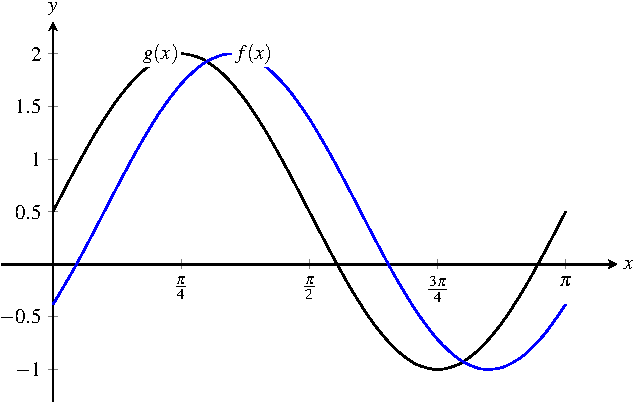
\includegraphics[scale=1.1]{image/13/sin-right-shift-pi-10.pdf}
\caption{%%
  Graphs of the sine functions
  $f(x) = \frac{3}{2} \sin(2x - \frac{\pi}{5}) + \frac{1}{2}$ and
  $g(x) = \frac{3}{2} \sin(2x) + \frac{1}{2}$.  The graph of $f(x)$ is
  obtained by shifting the graph of $g(x)$ along the horizontal axis
  by $\pi/10$ units to the right.
}
\label{fig:trigonometric:sin_right_shift_pi_10}
\end{figure}

\solutionpart{subeg:trigonometric:sin_right_shift_pi_10_graph}
Your $c$ value is $c = 2$.  The period of both $f(x)$ and $g(x)$ is
$2\pi / \absoluteValue{c} = 2\pi/2 = \pi$.
\Figure{fig:trigonometric:sin_right_shift_pi_10} shows graphs of
$f(x)$ and $g(x)$ from $x = 0$ to $x = \pi$.
\end{solution}

\begin{exercise}
Consider the function $f(x) = \cos(\frac{3}{2}x - \frac{5\pi}{2})$.
%%
\begin{packedenum}
\item\label{subex:trigonometric:cos_right_shift_standard_form}
  Write $f(x)$ in the form $f(x) = \cos\bigparen{c (x - h)}$.

\item\label{subex:trigonometric:cos_right_shift_5pi_3}
  Describe the graph of the function $f(x)$.

\item\label{subex:trigonometric:cos_right_shift_graph}
  Let $g(x) = \cos(cx)$ be the function $f(x)$ that has not been
  shifted horizontally.  On the same set of axes, graph $f(x)$ and
  $g(x)$ from $x = 0$ to $x = p$, where $p$ is the period of both
  $f(x)$ and $g(x)$.
\end{packedenum}
\end{exercise}

\ifbool{showSolution}{
\begin{solution}
\solutionpart{subex:trigonometric:cos_right_shift_standard_form}
To write $f(x) = \cos(\frac{3}{2}x - \frac{5\pi}{2})$ in the form
$f(x) = \cos\bigparen{c (x - h)}$, you must factorise the ratio
$\frac{3}{2}$.  Doing so results in the expression
\[
\frac{3}{2}x - \frac{5\pi}{2}
=
\frac{3}{2} \parenthesis*{x - \frac{5\pi}{3}}
\]
which can be used to write $f(x)$ as
%%
\begin{align*}
f(x)
&=
\cosp{\frac{3}{2}x - \frac{5\pi}{2}} \\[4pt]
&=
\cosp{\frac{3}{2} \parenthesis*{x - \frac{5\pi}{3}}}
\end{align*}
%%
where $h = \frac{5\pi}{3}$.

\solutionpart{subex:trigonometric:cos_right_shift_5pi_3}
Let $g(x) = \cos(\frac{3}{2} x)$.  The graph of $f(x)$ is obtained
by shifting the graph of $g(x)$ along the horizontal axis.  The amount
of horizontal shift is $\frac{5\pi}{3}$ units to the right.

\begin{figure}[!htbp]
\centering
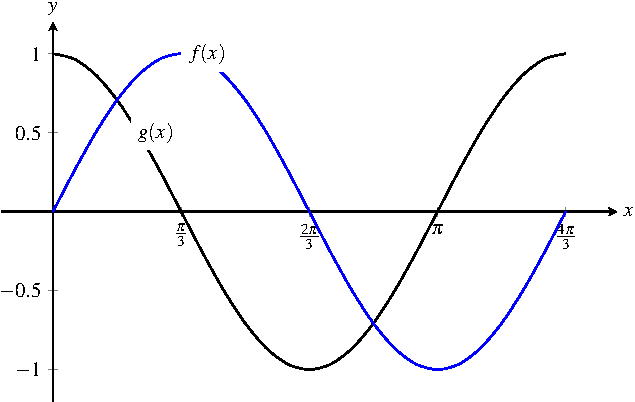
\includegraphics[scale=1.1]{image/13/cos-right-shift-5pi-3.pdf}
\caption{%%
  Graphs of the functions $f(x) = \cos(\frac{3}{2}x - \frac{5\pi}{2})$
  and $g(x) = \cos(\frac{3}{2} x)$ from $x = 0$ to
  $x = \frac{4\pi}{3}$.  The graph of $f(x)$ is obtained by shifting
  the graph of $g(x)$ by $\frac{5\pi}{3}$ units to the right.
}
\label{fig:trigonometric:cos_right_shift_5pi_3}
\end{figure}

\solutionpart{subex:trigonometric:cos_right_shift_graph}
Your $c$ value is $c = \frac{3}{2}$.  The period of both $f(x)$ and
$g(x)$ can be written as
%%
\begin{align*}
\frac{2\pi}{\absoluteValue{c}}
&=
\frac{2\pi}{3/2} \\[4pt]
&=
2\pi \times \frac{2}{3} \\[4pt]
&=
\frac{4\pi}{3}.
\end{align*}
%%
\Figure{fig:trigonometric:cos_right_shift_5pi_3} shows graphs of
$f(x)$ and $g(x)$ from $x = 0$ to $x = \frac{4\pi}{3}$.
\end{solution}
}{}

\begin{table}[!htbp]
\centering
\begin{tabular}{ccccccccccccc} \toprule
Month & Jan  & Feb  & Mar  & Apr  & May & Jun & Jul & Aug & Sep & Oct & Nov  & Dec \\
Mean  & 14.3 & 14.6 & 13.2 & 10.8 & 8.7 & 6.9 & 6   & 6.7 & 8   & 9.6 & 11.2 & 13  \\\bottomrule
\end{tabular}

\caption{%%
  The mean minimum temperature~($\degreec{}$) of each month for the
  city of Melbourne, Victoria, Australia.  The mean was calculated
  using temperature data for the years from $1855$ to $2015$.  The
  mean temperatures are provided by the Bureau of Meteorology of
  Australia.
}
\label{tab:trigonometry:mean_min_temperature}
\end{table}

\begin{exercise}
\textbf{Mean minimum temperature.}
\Table{tab:trigonometry:mean_min_temperature} shows the mean minimum
temperature~($\degreec{}$) for Melbourne for each month of the
year.\footnote{
  The data are available at
  \url{http://web.archive.org/web/20180709173611/http://www.bom.gov.au/climate/averages/tables/cw_086071.shtml},
  accessed 2018-07-09.
}
%%
\begin{packedenum}
\item\label{subex:trigonometric:mean_min_temperature_graph}
  As in \Part{subeg:trigonometric:mean_max_temperature_graph} of
  \Example{eg:trigonometric:mean_maximum_temperature}, associate each
  month of the year with a value from $0$ to $2\pi$.  Produce a
  scatter plot of the data in
  \Table{tab:trigonometry:mean_min_temperature}, where the horizontal
  axis represents a time of the year and the vertical axis represents
  the mean minimum temperature~($\degreec{}$).  Explain what you
  notice about the graph.

\item\label{subex:trigonometric:mean_min_temperature_cos}
  Suppose that the data in
  \Table{tab:trigonometry:mean_min_temperature} can be modelled as a
  cosine function of the form $f(x) = a \cos(cx) + b$, where $x$
  represents a time of the year and $f(x)$ represents the mean minimum
  temperature~($\degreec{}$) at $x$.  As in
  \Example{eg:trigonometric:mean_maximum_temperature}, use the data to
  estimate the values of $\triple{a}{b}{c}$.  You may assume that the
  period of $f(x)$ is $2\pi$ and $c > 0$.  Graph $f(x)$ together with
  the scatter plot
  from \Part{subex:trigonometric:mean_min_temperature_graph}.
  Calculate the root mean square error~(RMSE) and coefficient of
  determination $R^2$ of $f(x)$.

\item\label{subex:trigonometric:mean_min_temperature_cos_right_shift}
  Notice in \Table{tab:trigonometry:mean_min_temperature} that the
  temperature starts with $14.3$, followed by the highest value of
  $14.6$.  This suggests that the data can be modelled as a cosine
  function that has been right-shifted.  Suppose that the data in
  \Table{tab:trigonometry:mean_min_temperature} can be modelled as a
  function of the form $g(x) = a \cos\bigparen{c(x - h)} + b$.  Use
  the data in \Table{tab:trigonometry:mean_min_temperature} to
  estimate the values of $\quadruple{a}{b}{c}{h}$.  You may assume
  that the period of $g(x)$ is $2\pi$ and that $c > 0$.  Graph $g(x)$
  together with the graph
  from \Part{subex:trigonometric:mean_min_temperature_cos}.  Calculate
  the RMSE and $R^2$ of $g(x)$.  Use the values of the RMSE and $R^2$
  to help you decide which one of the functions $f(x)$ and $g(x)$ is
  better than the other at modelling the data in
  \Table{tab:trigonometry:mean_min_temperature}.
\end{packedenum}
\end{exercise}

\ifbool{showSolution}{
\begin{solution}
\solutionpart{subex:trigonometric:mean_min_temperature_graph}
\Figure{fig:trigonometric:mean_min_temperature} shows a scatter plot
of the data in \Table{tab:trigonometry:mean_min_temperature}.  The
graph shows that the black dots seem to follow the graph of a cosine
function that has been shifted to the right.

\begin{figure}[!htbp]
\centering
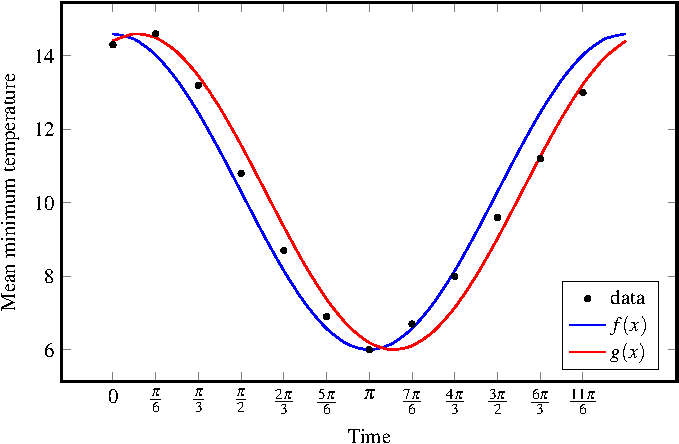
\includegraphics[scale=1.1]{image/13/mean-min-temperature.pdf}
\caption{%%
  The mean minimum temperature~($\degreec{}$) for Melbourne.  Each
  tick on the horizontal axis represents a month of the year.  So $0$
  corresponds to January, $\frac{\pi}{6}$ corresponds to February, and
  so on.  The black dots show the data in
  \Table{tab:trigonometry:mean_min_temperature}.  The blue curve is a
  graph of \Equation{eqn:trigonometric:mean_min_temperature_cos}.  The
  red curve is a graph of
  \Equation{eqn:trigonometric:mean_min_temperature_cos_right_shift}.
}
\label{fig:trigonometric:mean_min_temperature}
\end{figure}

\solutionpart{subex:trigonometric:mean_min_temperature_cos}
Suppose that the data in \Table{tab:trigonometry:mean_min_temperature}
can be modelled as a function of the form $f(x) = a \cos(cx) + b$.
The value $b$ of the midline is the mean of the minimum and maximum
values in \Table{tab:trigonometry:mean_min_temperature}.  The minimum
and maximum values are $6$ and $14.6$, respectively, hence the value
of the midline is
\[
b
=
\frac{6 + 14.6}{2}
=
10.3.
\]
The amplitude $a$ is the absolute value of the difference between the
maximum value and the value of the midline.  Thus you have
\[
a
=
\absoluteValue{14.6 - 10.3}
=
\absoluteValue{4.3}
=
4.3.
\]
Since the period of $f(x)$ is assumed to be $2\pi$, then the period
can be written as $\frac{2\pi}{\absoluteValue{c}} = 2\pi$.  Multiply
both sides by $\absoluteValue{c}$ to get
$2\pi = 2\pi\absoluteValue{c}$.  Solving the latter equation for
$\absoluteValue{c}$ shows that $\absoluteValue{c} = 1$.  As you have
assumed that $c > 0$, it follows that $c = 1$.  Thus the function
$f(x)$ can be written as
%%
\begin{equation}
\label{eqn:trigonometric:mean_min_temperature_cos}
f(x)
=
4.3 \cos x + 10.3
\end{equation}
%%
and graphed in \Figure{fig:trigonometric:mean_min_temperature}.  The
function $f(x)$ has a root mean square error of
$\text{RMSE} \approx 0.631172$.  The sum of squared errors is
$\text{SSE} \approx 4.780541$ and the total sum of squares is
$\text{TSS} = 102.57$.  Then the coefficient of determination of
$f(x)$ is
%%
\begin{align*}
R^2
&=
1 - \frac{\text{SSE}}{\text{TSS}} \\[4pt]
&\approx
0.953392.
\end{align*}

\solutionpart{subex:trigonometric:mean_min_temperature_cos_right_shift}
Suppose that the data in \Table{tab:trigonometry:mean_min_temperature}
can be modelled as a cosine function of the form
$g(x) = a \cos\bigparen{c (x - h)} + b$.  Notice that the graph of
$g(x)$ can be obtained by shifting the graph of $f(x)$ along the
horizontal axis.  The amount of horizontal shift is $h$ units to the
right.  Since the data in
\Table{tab:trigonometry:mean_min_temperature} starts with $14.3$
followed by the maximum of $14.6$, you may assume that the amount by
which to right shift is
%%
\begin{align*}
h
&=
\absoluteValue{14.3 - 14.6} \\[4pt]
&=
\absoluteValue{-0.3} \\[4pt]
&=
0.3.
\end{align*}
%%
Thus $g(x)$ can be written as
%%
\begin{equation}
\label{eqn:trigonometric:mean_min_temperature_cos_right_shift}
g(x)
=
4.3 \cos(x - 0.3) + 10.3
\end{equation}
%%
and graphed in \Figure{fig:trigonometric:mean_min_temperature}.  The
function $g(x)$ has a root mean square error of
$\text{RMSE} \approx 0.485174$.  The sum of squared errors is
$\text{SSE} \approx 2.824728$ and the total sum of squares is
$\text{TSS} = 102.57$.  The coefficient of determination of $g(x)$ is
%%
\begin{align*}
R^2
&=
1 - \frac{\text{SSE}}{\text{TSS}} \\[4pt]
&\approx
0.972460.
\end{align*}
%%
Notice that the RMSE of $g(x)$ is lower than the RMSE of $f(x)$.
Furthermore, $g(x)$ has a higher value of $R^2$ than does $f(x)$.
Based on the values of the RMSE and $R^2$, you may conclude that
$g(x)$ is better than $f(x)$ at modelling the data in
\Table{tab:trigonometry:mean_min_temperature}.
\end{solution}
}{}

\begin{example}
\textbf{Left shift.}
Consider the function
$f(x) = \cos(\frac{1}{2} x + \frac{2}{3}) + \frac{3}{4}$.
%%
\begin{packedenum}
\item\label{subeg:trigonometric:cos_left_shift_4third_standard_form}
  Write $f(x)$ in the form $f(x) = \cos\bigparen{c(x - h)} + b$.

\item\label{subeg:trigonometric:cos_left_shift_4third_describe}
  Describe the graph of the function $f(x)$.

\item\label{subeg:trigonometric:cos_left_shift_4third_graph}
  Let $g(x) = \cos(cx) + b$ be the function $f(x)$ that has not been
  shifted horizontally.  On the same set of axes, graph $f(x)$ and
  $g(x)$ from $x = 0$ to $x = p$, where $p$ is the period of both
  $f(x)$ and $g(x)$.
\end{packedenum}
\end{example}

\begin{solution}
\solutionpart{subeg:trigonometric:cos_left_shift_4third_standard_form}
To write $f(x)$ in the form $f(x) = \cos\bigparen{c(x - h)} + b$, you
must factorise the ratio $\frac{1}{2}$.  Note that you have
$\frac{1}{2} x + \frac{2}{3} = \frac{1}{2} (x + \frac{4}{3})$.  Use
the latter expression to write $f(x)$ as
%%
\begin{align*}
f(x)
&=
\cosp{\frac{1}{2} x + \frac{2}{3}} + \frac{3}{4} \\[4pt]
&=
\cosp{\frac{1}{2} \parenthesis*{x + \frac{4}{3}}} + \frac{3}{4}
\end{align*}
%%
where $h = -\frac{4}{3}$.

\solutionpart{subeg:trigonometric:cos_left_shift_4third_describe}
Let $g(x) = \cos(\frac{1}{2} x) + \frac{3}{4}$.  The graph of $f(x)$
is obtained by shifting the graph of $g(x)$ along the horizontal axis.
The amount of horizontal shift is $\frac{4}{3}$ units to the left.

\begin{figure}[!htbp]
\centering
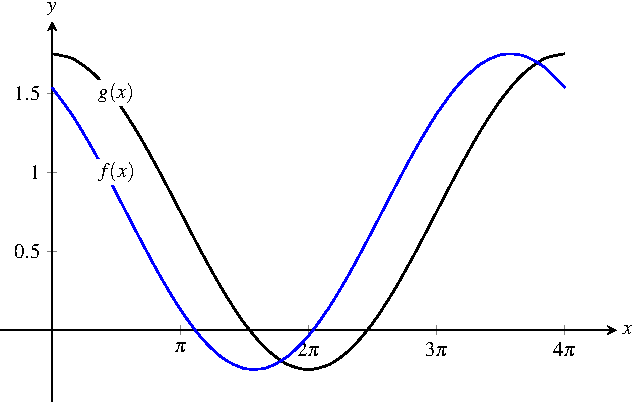
\includegraphics[scale=1.1]{image/13/cos-left-shift-4third.pdf}
\caption{%%
  Graphs of the functions
  $f(x) = \cos(\frac{1}{2} x + \frac{2}{3}) + \frac{3}{4}$ and
  $g(x) = \cos(\frac{1}{2} x) + \frac{3}{4}$ from $x = 0$ to
  $x = 4\pi$.
}
\label{fig:trigonometric:cos_left_shift_4third}
\end{figure}

\solutionpart{subeg:trigonometric:cos_left_shift_4third_graph}
Your $c$ value is $c = \frac{1}{2}$.  The period of both $f(x)$ and
$g(x)$ be can be written as the expression
%%
\begin{align*}
\frac{2\pi}{\absoluteValue{c}}
&=
\frac{2\pi}{1/2} \\[4pt]
&=
2\pi \times 2 \\[4pt]
&=
4\pi.
\end{align*}
%%
\Figure{fig:trigonometric:cos_left_shift_4third} shows graphs of
$f(x)$ and $g(x)$.
\end{solution}

\begin{exercise}
Consider the function
$f(x) = \frac{3}{5} \sin(3x + \frac{2\pi}{3}) + \frac{1}{4}$.
%%
\begin{packedenum}
\item\label{subex:trigonometric:sin_left_shift_2pi_9_standard_form}
  Write $f(x)$ in the form $f(x) = a \sin\bigparen{c (x - h)} + b$.

\item\label{subex:trigonometric:sin_left_shift_2pi_9_describe}
  Describe the graph of the function $f(x)$.

\item\label{subex:trigonometric:sin_left_shift_2pi_9_graph}
  Let $g(x) = a \sin(cx) + b$ be the function $f(x)$ that has not been
  shifted horizontally.  On the same set of axes, graph $f(x)$ and
  $g(x)$ from $x = 0$ to $x = p$, where $p$ is the period of both
  $f(x)$ and $g(x)$.

\item\label{subex:trigonometric:sin_left_shift_2pi_9_frequency}
  Calculate the frequency of both $f(x)$ and $g(x)$.
\end{packedenum}
\end{exercise}

\ifbool{showSolution}{
\begin{solution}
\solutionpart{subex:trigonometric:sin_left_shift_2pi_9_standard_form}
To write $f(x)$ in the form $f(x) = a \sin\bigparen{c (x - h)} + b$,
you must factorise the $3$ in the expression $3x + \frac{2\pi}{3}$.
Doing so yields the factorisation
\[
3x + \frac{2\pi}{3}
=
3 \parenthesis*{x + \frac{2\pi}{9}}
\]
which can be used to write $f(x)$ as
%%
\begin{align*}
f(x)
&=
\frac{3}{5} \sinp{3x + \frac{2\pi}{3}} + \frac{1}{4} \\[4pt]
&=
\frac{3}{5} \sinp{3 \parenthesis*{x + \frac{2\pi}{9}}} + \frac{1}{4}.
\end{align*}
%%
From the latter expression you have $h = -\frac{2\pi}{9}$.

\solutionpart{subex:trigonometric:sin_left_shift_2pi_9_describe}
Let $g(x) = \frac{3}{5} \sin(3x) + \frac{1}{4}$.  The graph of $f(x)$
is obtained by shifting the graph of $g(x)$ along the horizontal
axis.  The amount of horizontal shift is $\frac{2\pi}{9}$ units to the
left.

\begin{figure}[!htbp]
\centering
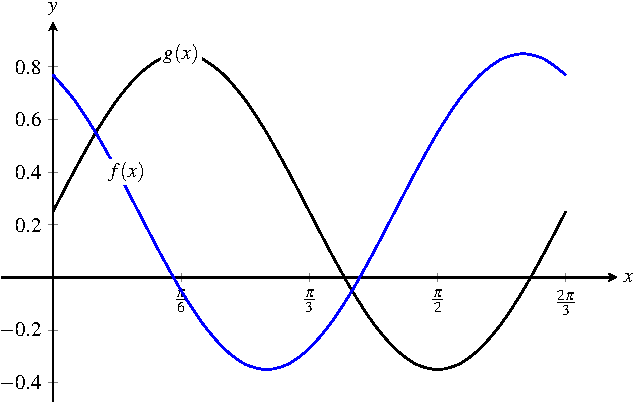
\includegraphics[scale=1.1]{image/13/sin-left-shift-2pi-9.pdf}
\caption{%%
  Graphs of the sine functions
  $f(x) = \frac{3}{5} \sin(3x + \frac{2\pi}{3}) + \frac{1}{4}$ and
  $g(x) = \frac{3}{5} \sin(3x) + \frac{1}{4}$ from $x = 0$ to
  $x = \frac{2\pi}{3}$.
}
\label{fig:trigonometric:sin_left_shift_2pi_9}
\end{figure}

\solutionpart{subex:trigonometric:sin_left_shift_2pi_9_graph}
Your $c$ value is $c = 3$.  The period of both $f(x)$ and $g(x)$ is
$p = 2\pi / 3$.  \Figure{fig:trigonometric:sin_left_shift_2pi_9} shows
graphs of $f(x)$ and $g(x)$ from $x = 0$ to $x = \frac{2\pi}{3}$.

\solutionpart{subex:trigonometric:sin_left_shift_2pi_9_frequency}
The frequency of both $f(x)$ and $g(x)$ can be calculated as
%%
\begin{align*}
\frac{1}{p}
&=
\frac{1}{2\pi/3} \\[4pt]
&=
1 \times \frac{3}{2\pi} \\[4pt]
&=
\frac{3}{2\pi}.
\end{align*}
%%
Thus $f(x)$ and $g(x)$ both have a frequency of $\frac{3}{2\pi}$.
\end{solution}
}{}


\newpage
%%%%%%%%%%%%%%%%%%%%%%%%%%%%%%%%%%%%%%%%%%%%%%%%%%%%%%%%%%%%%%%%%%%%%%%%%%%

\section*{Problem}

\begin{problem}
\item Read the following paper by David M. Bressoud:
  \emph{Historical Reflections on Teaching Trigonometry}.\footnote{
    The paper is available at
    \url{https://www.jstor.org/stable/20876798}.
  }

\item\label{prob:trigonometric:cannon_cliff}
  \emph{Projectile motion.}
  You have learnt that when an object is launched upward and allowed
  to travel freely along the vertical direction, the motion of the
  object is an example of free fall.  Now consider the case of an
  object that moves in both the horizontal and vertical directions.
  Examples include a car that runs off a cliff\footnote{
    See the video at
    \url{https://youtu.be/XKwrMzcnxmg}.
  }
  or a bomb that is dropped from an aeroplane.\footnote{
    See the video at
    \url{https://youtu.be/IhY9LBNVroo}.
  }
  The object will travel horizontally and at the same time it is being
  pulled towards the centre of the Earth by the force of gravity.  The
  path that the object traces out is parabolic and the movement of the
  object is an example of \emph{projectile motion}.  As an example,
  suppose that a cannon is placed at the top of a cliff.  Let $h > 0$
  be the vertical distance~(in metres) from the top of the cliff to
  ground level.  The cannon fires a cannonball along the horizontal
  direction at a velocity of $v_x$ metres per second.
  %%
  \begin{packedenum}
  \item\label{subprob:trigonometric:cannon_cliff_horizontal_displacement}
    Let $t \geq 0$ be the amount of time in seconds since the
    cannonball was fired.  After $t$ seconds, the cannonball would
    have covered a horizontal distance of $v_xt$ metres.  Suppose that
    the cannonball was fired along the horizontal direction at a
    velocity of $v_x = 10$~metres per second.  If $X(t)$ represents
    the amount of horizontal distance that the cannonball covered
    after $t$ seconds, write an equation for $X(t)$.  Graph your
    function $X(t)$ from $t = 0$ to $t = 3$.  How long must you wait
    for the cannonball to have covered a horizontal distance of $25$
    metres?

  \item\label{subprob:trigonometric:cannon_cliff_vertical_displacement}
    The cannonball is propelled only along the horizontal direction.
    As the cannonball travels along the horizontal direction, it is
    acted upon by the force of gravity, which is the constant of
    $g = 9.8$~metres per second squared.  Recall that when an object
    travels vertically under free fall, the vertical distance $Y(t)$
    in metres between the object and ground level after $t$ seconds
    can be approximated as the quadratic function
    $Y(t) = -\frac{1}{2} gt^2 + v_yt + h$, where air drag has been
    ignored.  Here, $v_y$ is the initial velocity with which the
    object is launched along the vertical direction and $h$ is the
    initial height in metres between the object and ground level.
    Since the cannonball is propelled only along the horizontal
    direction, the vertical velocity is $v_y = 0$.  Thus you can
    simplify $Y(t)$ as
    %%
    \begin{equation}
    \label{eqn:trigonometric:cannon_cliff_vertical_displacement}
    Y(t)
    =
    h - \frac{1}{2}gt^2.
    \end{equation}
    %%
    In other words, at any time $t \geq 0$ after the cannonball has
    been fired the function $X(t)$ describes the horizontal
    distance~(metres) from the cannonball to the tip of the cannon.
    Furthermore, the function $Y(t)$ describes the vertical
    distance~(metres) from the cannonball to ground level.  Suppose
    that the distance from the top of the cliff to ground level is
    $50$~metres.  Produce a graph of
    \Equation{eqn:trigonometric:cannon_cliff_vertical_displacement}
    from time $t = 0$ to $t = 3.5$~seconds.  At $t = 2$ seconds after
    the cannonball has been fired, how far in metres is the cannonball
    to ground level?  How much time is required for the cannonball to
    be at a vertical distance of $25$~metres from ground level?

  \item\label{subprob:trigonometric:cannon_cliff_time_to_ground}
    Let the value of $h$ be as
    in \Part{subprob:trigonometric:cannon_cliff_vertical_displacement}
    and let $Y(t)$ be defined by
    \Equation{eqn:trigonometric:cannon_cliff_vertical_displacement}.
    Produce a table that has three columns and as many rows as
    necessary.  Going from left to right, the first column has the
    header $t$ and lists the time from $t = 0$ to $t = 3.5$ seconds
    with an increment of $0.1$ seconds.  The second column lists
    values of $X(t)$.  Finally, the third column lists values of
    $Y(t)$.  Graph values of $X(t)$ versus values of $Y(t)$, where
    values of $X(t)$ are on the horizontal axis and values of $Y(t)$
    are on the vertical axis.  Describe your graph.  After being
    fired, calculate the amount of time~(in seconds) required for the
    cannonball to land on the ground.  When the cannonball lands on
    the ground, determine the horizontal distance from the cannonball
    to the tip of the cannon.

  \item\label{subprob:trigonometric:cannon_cliff_intersection}
    On the same set of axes, graph the functions $X(t)$ and $Y(t)$
    from $t = 0$ to $t = \sqrt{50 / 4.9}$.  Use your graph to explain
    why, after the cannonball is fired, there is a positive value of
    $t$ such that $X(t) = Y(t)$.  Explain what the latter equality
    means.  Calculate a positive value of $t$ such that
    $X(t) = Y(t)$.
  \end{packedenum}
\ifbool{showSolution}{
\begin{solution}
\solutionpart{subprob:trigonometric:cannon_cliff_horizontal_displacement}
Let $X(t)$ be the horizontal distance in metres that the cannonball
covers $t$ seconds after it is being fired.  Then you have the
expression $X(t) = v_x t$, where $v_x$ is the velocity with which the
cannonball was fired.  Since you have assumed that $v_x = 10$ metres
per second, then $X(t)$ can be written as
%%
\begin{equation}
\label{eqn:trigonometric:horizontal_distance_to_cannon}
X(t)
=
10t.
\end{equation}
%%
\Figure{fig:trigonometric:cannon_cliff_horizontal_displacement} shows
a graph of $X(t)$ from $t = 0$ to $t = 3$.

\begin{figure}[!htbp]
\centering
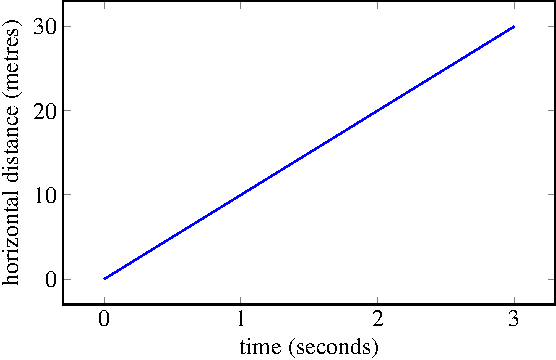
\includegraphics[scale=1]{image/13/cannonball-horizontal-displacement.pdf}
\caption{%%
  The horizontal distance~(metres) that a cannonball covers $t$
  seconds after being fired.
}
\label{fig:trigonometric:cannon_cliff_horizontal_displacement}
\end{figure}

Suppose that the cannonball has covered a horizontal distance of
$25$~metres and you want to calculate the amount of time required to
cover the given distance.  You can write the problem as the equation
$X(t) = 25$ or equivalently as $10t = 25$.  Solving for $t$ shows that
you have $t = 25 / 10 = 2.5$.  That is, you must wait $2.5$ seconds in
order for the cannonball to travel a horizontal distance of $25$
metres.

\begin{figure}[!htbp]
\centering
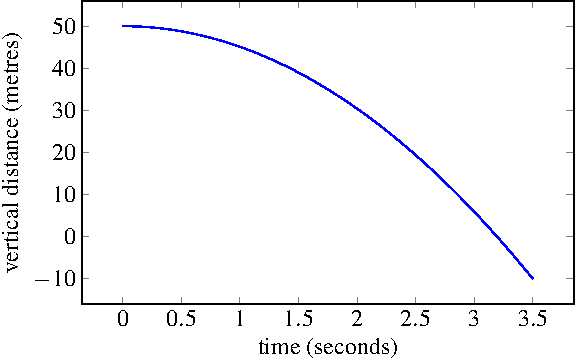
\includegraphics[scale=1]{image/13/cannonball-vertical-displacement.pdf}
\caption{%%
  The distance $Y(t)$ from the cannonball to ground level at $t$
  seconds after the cannonball has been fired.
}
\label{fig:trigonometric:cannon_cliff_vertical_displacement}
\end{figure}

\solutionpart{subprob:trigonometric:cannon_cliff_vertical_displacement}
You have $g = 9.8$~metres per second squared and $h = 50$~metres.
Then \Equation{eqn:trigonometric:cannon_cliff_vertical_displacement}
can be simplified to
%%
\begin{equation}
\label{eqn:trigonometric:cannon_vertical_distance_h_50}
\begin{aligned}
Y(t)
&=
50 - \frac{9.8}{2} t^2 \\[4pt]
&=
50 - 4.9 t^2.
\end{aligned}
\end{equation}
%%
The latter expression is graphed in
\Figure{fig:trigonometric:cannon_cliff_vertical_displacement} from
$t = 0$ to $t = 3.5$.  When $t = 2$, you have
%%
\begin{align*}
Y(2)
&=
50 - 4.9 \cdot 2^2 \\[4pt]
&=
30.4.
\end{align*}
%%
In other words, at $t = 2$~seconds after being fired the cannonball
would be at a distance of $30.4$~metres to ground level.

Now suppose that the cannonball is at a distance of $25$~metres to
ground level.  To calculate the amount of time required, substitute
the expression $Y(t) = 25$ into
\Equation{eqn:trigonometric:cannon_vertical_distance_h_50} to obtain
the expression $50 - 4.9t^2 = 25$, which can also be written as
$4.9t^2 = 50 - 25$.  The last equation can be simplified to
$4.9t^2 = 25$.  Divide both sides by $4.9$ and then solve for $t$ to
obtain $t = \pm\sqrt{25 / 4.9}$.  Since $-\sqrt{25 / 4.9}$ is
negative, you may ignore this solution.  Conclude that at
approximately $t = \sqrt{25 / 4.9} \approx 2.26$~seconds after being
fired, the cannonball would be at a distance of $25$~metres to ground
level.

\begin{table}[!htbp]
\centering
\begin{tabular}{ccc} \toprule
$t$   & $X(t)$ & $Y(t)$   \\\midrule
$0.0$ & $0$    & $50.000$ \\
$0.1$ & $1$    & $49.951$ \\
$0.2$ & $2$    & $49.804$ \\
$0.3$ & $3$    & $49.559$ \\
$0.4$ & $4$    & $49.216$ \\
$0.5$ & $5$    & $48.775$ \\
$0.6$ & $6$    & $48.236$ \\
$0.7$ & $7$    & $47.599$ \\
$0.8$ & $8$    & $46.864$ \\
$0.9$ & $9$    & $46.031$ \\
$1.0$ & $10$   & $45.100$ \\
$1.1$ & $11$   & $44.071$ \\
$1.2$ & $12$   & $42.944$ \\
$1.3$ & $13$   & $41.719$ \\
$1.4$ & $14$   & $40.396$ \\
$1.5$ & $15$   & $38.975$ \\
$1.6$ & $16$   & $37.456$ \\
$1.7$ & $17$   & $35.839$ \\
$1.8$ & $18$   & $34.124$ \\
$1.9$ & $19$   & $32.311$ \\
$2.0$ & $20$   & $30.400$ \\
$2.1$ & $21$   & $28.391$ \\
$2.2$ & $22$   & $26.284$ \\
$2.3$ & $23$   & $24.079$ \\
$2.4$ & $24$   & $21.776$ \\
$2.5$ & $25$   & $19.375$ \\
$2.6$ & $26$   & $16.876$ \\
$2.7$ & $27$   & $14.279$ \\
$2.8$ & $28$   & $11.584$ \\
$2.9$ & $29$   & $8.791$  \\
$3.0$ & $30$   & $5.900$  \\
$3.1$ & $31$   & $2.911$  \\
$3.2$ & $32$   & $-0.176$ \\
$3.3$ & $33$   & $-3.361$ \\
$3.4$ & $34$   & $-6.644$ \\
$3.5$ & $35$   & $-10.025$ \\\bottomrule
\end{tabular}

\caption{%%
  The path of the cannonball after it is fired from the cannon.
  Values of $X(t)$ give the horizontal distances~(metres) from the
  cannonball to the tip of the cannon at $t$ seconds after being
  fired.  Similarly, values of $Y(t)$ represent the vertical
  distances~(metres) from the cannonball to ground level at $t$
  seconds after being fired.  Some values in the right-most column
  have been rounded to three decimal places.
}
\label{tab:trigonometric:cannon_cliff_path}
\end{table}

\begin{figure}[!htbp]
\centering
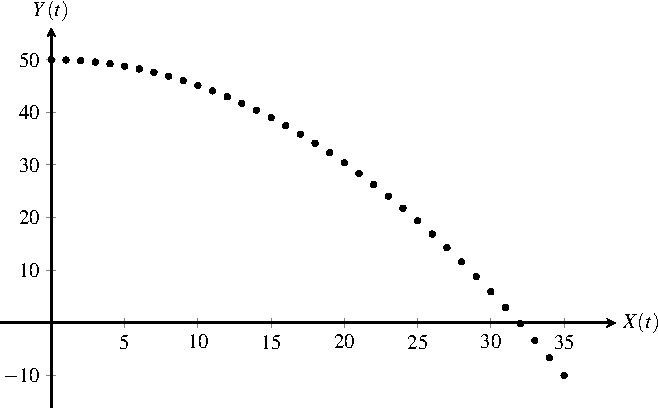
\includegraphics[scale=1.1]{image/13/cannonball-trajectory.pdf}
\caption{%%
  The path of the cannonball after it is fired from the cannon.  The
  horizontal axis represents the horizontal distance between the
  cannonball and the cannon.  The vertical axis represents the
  vertical distance from the cannonball to ground level.  All
  distances are measured in metres.
}
\label{fig:trigonometric:cannon_cliff_trajectory}
\end{figure}

\solutionpart{subprob:trigonometric:cannon_cliff_time_to_ground}
\Table{tab:trigonometric:cannon_cliff_path} shows values of $X(t)$ and
$Y(t)$ from $t = 0$ to $t = 3.5$ at an increment of $0.1$ seconds.
\Figure{fig:trigonometric:cannon_cliff_trajectory} shows a scatter
plot of values of $X(t)$ versus values of $Y(t)$.  The horizontal axis
represents the horizontal distance $X(t)$ from the cannonball to the
tip of the cannon, while the vertical axis represents the vertical
distance $Y(t)$ from the cannonball to ground level.  Values of
$t \geq 0$ represent time in seconds since the cannonball was fired.
Since the cannon is at a vertical distance of $50$~metres from ground
level, the point $\tuple{0}{50}$ represents where the tip of the
cannon is located.  The horizontal axis represents the ground level
and the vertical axis represents the cliff.

Let's determine the amount of time required for the fired cannonball
to reach ground level.  You have the expression $Y(t) = 0$, which asks
for all values of $t$ such that the equation is true.  Substitute the
latter expression into
\Equation{eqn:trigonometric:cannon_vertical_distance_h_50} to obtain
$50 - 4.9 t^2 = 0$ or equivalently the expression $4.9t^2 = 50$.
Divide both sides by $4.9$ and solving for $t$ shows that you have
$t = \pm\sqrt{50 / 4.9}$.  Since $-\sqrt{50 / 4.9}$ is negative, you
may ignore this solution.  Therefore at approximately
$t = \sqrt{50 / 4.9} \approx 3.19$~seconds after being fired, the
cannonball would land on the ground.

Finally, let's calculate the horizontal distance from the cannonball
to the tip of the cannon when the cannonball reaches ground level.
The function $X(t)$ models the horizontal distance from the cannonball
to the tip of the cannon at $t$ seconds after being fired.  Since the
cannonball requires $\sqrt{50 / 4.9}$ seconds to reach ground level,
then you have $X(\sqrt{50 / 4.9}) \approx 31.94$.  That is, when the
cannonball lands on the ground, the cannonball would be at a
horizontal distance of approximately $31.94$~metres from the tip of
the cannon.

\begin{figure}[!htbp]
\centering
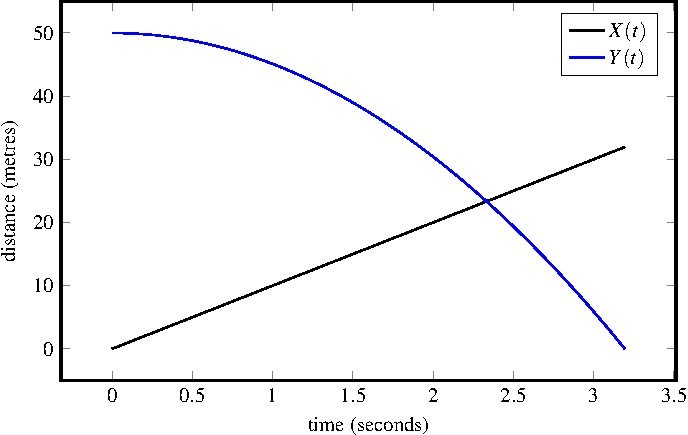
\includegraphics[scale=1.1]{image/13/cannonball-intersection.pdf}
\caption{%%
  The intersection of the functions $X(t)$ and $Y(t)$ as defined by
  \Equations{eqn:trigonometric:horizontal_distance_to_cannon}{eqn:trigonometric:cannon_vertical_distance_h_50},
  respectively.
}
\label{fig:trigonometric:cannonball_intersection}
\end{figure}

\solutionpart{subprob:trigonometric:cannon_cliff_intersection}
\Figure{fig:trigonometric:cannonball_intersection} shows the graphs of
\Equations{eqn:trigonometric:horizontal_distance_to_cannon}{eqn:trigonometric:cannon_vertical_distance_h_50}
on the same set of axes.  The figure clearly shows that the graphs of
the functions $X(t)$ and $Y(t)$ intersect each other at a positive
value of $t$.  The horizontal coordinate of the point of intersection
is bounded by the inequality $2 \leq t \leq 2.5$.  At the given
positive value of $t$, whatever it may be, you have the equality
$X(t) = Y(t)$.  The latter equality means that at $t$ seconds after
the cannonball is fired the horizontal distance $X(t)$ from the
cannonball to the tip of the cannon is the same as the vertical
distance $Y(t)$ from the cannonball to ground level.

Let's determine a positive value of $t$ such that $X(t) = Y(t)$.  Note
that the latter equality can be written as
$10t = 50 - 4.9t^2$ and moving everything to the left-hand side
results in the equation
\[
4.9t^2 + 10t - 50
=
0.
\]
The latter equation asks for the roots of the quadratic function
$f(t) = 4.9t^2 + 10t - 50$.  You have the discriminant
$\Delta = 10^2 - 4(4.9)(-50) = 1080$.  Using the quadratic formula,
the roots of $f(t)$ are
%%
\begin{align*}
t
&=
\frac{
  -10 \pm \sqrt{\Delta}
}{
  2(4.9)
} \\[4pt]
&=
\frac{
  -10 \pm \sqrt{1080}
}{
  9.8
}.
\end{align*}
%%
Note that
\[
t
=
\frac{
  -10 - \sqrt{1080}
}{
  9.8
}
\]
is a negative number, whereas
\[
t
=
\frac{
  -10 + \sqrt{1080}
}{
  9.8
}
\approx
2.332995.
\]
In other words, at approximately $t \approx 2.33$ seconds after the
cannonball is fired you have $X(t) = Y(t)$.
\end{solution}
}{}

\item\emph{Trajectory of a baseball.}
  You are standing at ground level.\footnote{
    See for example the video at
    \url{https://youtu.be/pXhIGo9179s}.
    A similar example is a cannon firing a cannonball at an angle; see
    the video at
    \url{https://youtu.be/1TOu4WLnb6k}.
    The same principles can also be found in the game
    ``Angry Birds''; see the video at
    \url{https://youtu.be/WrNP1oAmDGw}.
  }
  Suppose that ground level is interpreted as the horizontal axis and
  that vertical height is interpreted as the vertical axis.  You hit a
  baseball at an angle of $\varphi$ radians with respect to the
  positive half of the horizontal axis.\footnote{
    Different angles will result in different trajectories for the
    baseball.  See the video at
    \url{https://youtu.be/N0H-rv9XFHk}.
  }
  The ball is hit with an initial speed of $v \geq 0$ metres per
  second.  When the ball is hit, the distance from the ball to ground
  level is $h \geq 0$ metres.  The initial velocity of the baseball
  along the horizontal axis is $v_x = v \cos\varphi$ and the initial
  velocity along the vertical axis is $v_y = v \sin\varphi$.
  %%
  \begin{packedenum}
  \item\label{subprob:trigonometric:baseball_X(t)}
    Let $t \geq 0$ be the amount of time in seconds since the baseball
    was hit.  After $t$ seconds, the baseball would have covered a
    horizontal distance of $v_x t$ metres.  Suppose you hit the
    baseball with an initial speed of $v = 40$~metres per second at an
    angle of $\degree{45}$.  If $X(t)$ represents the amount of
    horizontal distance~(metres) that the baseball covers after $t$
    seconds, write an equation for $X(t)$.  Graph your function from
    $t = 0$ up to $t = 6$ seconds.  After you hit the baseball, how
    long must you wait for the baseball to cover a horizontal distance
    of $100$ metres?

  \item\label{subprob:trigonometric:baseball_Y(t)}
    As the baseball traces out its trajectory, the vertical distance
    from the baseball to ground level changes with time.  If $Y(t)$
    represents the vertical distance from the baseball to ground level
    at $t$ seconds after being hit, then you can write
    $Y(t) = -\frac{1}{2} g t^2 + v_y t + h$.  Here, you have ignored
    the effect of air drag and only consider the effect of gravity on
    the baseball, where $g$ is the gravitational constant.  As
    in \Part{subprob:trigonometric:baseball_X(t)}, suppose that you
    hit the baseball with an initial speed of $v = 40$ metres per
    second at an angle of $\degree{45}$.  Further suppose that when
    you hit the baseball, it is at a height of one metre to ground
    level.  Use the above information to write an equation for
    $Y(t)$.  Graph your function $Y(t)$ together with the graph
    from \Part{subprob:trigonometric:baseball_X(t)}.  After you hit
    the baseball, how long must you wait for the baseball to be at a
    vertical distance of $40$ metres to ground level?

  \item\label{subprob:trigonometric:baseball_trajectory}
    Let $X(t)$ and $Y(t)$ be as
    in \Parts{subprob:trigonometric:baseball_X(t)}{subprob:trigonometric:baseball_Y(t)},
    respectively.  Construct a table similar to the table in
    \Subproblem{prob:trigonometric:cannon_cliff}{subprob:trigonometric:cannon_cliff_time_to_ground}.
    Use the time values from $t = 0$ to $t = 6$ seconds with an
    increment of $0.25$ seconds.  Graph values of $X(t)$ versus values
    of $Y(t)$.  Here, values of $X(t)$ and $Y(t)$ are on the
    horizontal and vertical axes, respectively.  Explain what you
    notice about the graph.  Using your graph, determine an
    approximate value for the maximum height above ground level that
    the baseball reaches after you hit the baseball.  When the
    baseball is at the given maximum height, use your graph to
    determine an approximate value for horizontal distance from the
    baseball to you.  When the baseball lands on the ground, determine
    an approximate distance between you and the baseball.

  \item\label{subprob:trigonometric:baseball_trajectory_30_degree}
    You hit a baseball at an angle of $\degree{30}$ with an initial
    speed of $50$ metres per second.  At the time that the baseball is
    hit, the ball is $1$ metre from ground level.  Calculate the
    amount of time~(seconds) required for the baseball to land on the
    ground.  When the baseball lands on the ground, determine the
    horizontal distance~(metres) from the baseball to its original
    position.
  \end{packedenum}
\ifbool{showSolution}{
\begin{solution}
\solutionpart{subprob:trigonometric:baseball_X(t)}
You have $X(t) = v_x t$ and $v = 40$~metres per second.  The angle of
$\degree{45}$ is equivalent to $\varphi = \frac{\pi}{4}$ radians.
Since $v_x = v \cos\varphi$, you can write
$X(t) = (v \cos\varphi) t$.  Substitute in the values for $v$ and
$\varphi$ and you obtain
%%
\begin{equation}
\label{eqn:trigonometric:baseball_x_displacement}
\begin{aligned}
X(t)
&=
\parenthesis*{40 \cos\frac{\pi}{4}} t \\[4pt]
&=
40 \frac{\sqrt{2}}{2} t \\[4pt]
&=
20 \sqrt{2} t
\end{aligned}
\end{equation}
%%
which is graphed in
\Figure{fig:trigonometric:baseball_x_y_displacement}.  To calculate
the amount of time required for the baseball to cover a horizontal
distance of $100$ metres, consider the equation
$100 = 20 \sqrt{2} t$.  Divide both sides by $20 \sqrt{2}$ and you end
up with
\[
t
=
\frac{100}{20 \sqrt{2}}
=
\frac{5}{\sqrt{2}}
\approx
3.5355.
\]
That is, after you hit the baseball you must wait approximately $3.5$
seconds in order for the baseball to cover a horizontal distance of
$100$ metres.

\begin{figure}[!htbp]
\centering
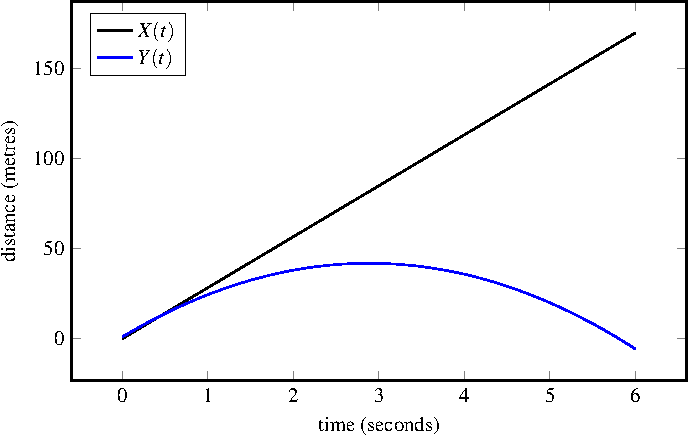
\includegraphics[scale=1.1]{image/13/baseball-x-y-displacement.pdf}
\caption{%%
  The horizontal and vertical distances~(in metres) of the baseball
  after it is hit.  The black line shows the horizontal distance
  $X(t)$ that the baseball covers at $t$ seconds after being hit.  The
  blue curve shows the vertical distance $Y(t)$ from the baseball to
  ground level at $t$ seconds after being hit.  The functions $X(t)$
  and $Y(t)$ are defined in
  \Equations{eqn:trigonometric:baseball_x_displacement}{eqn:trigonometric:baseball_y_displacement},
  respectively.
}
\label{fig:trigonometric:baseball_x_y_displacement}
\end{figure}

\solutionpart{subprob:trigonometric:baseball_Y(t)}
You have the expression $Y(t) = -\frac{1}{2} g t^2 + v_y t + h$.
Furthermore, you have the gravitational constant of $g = 9.8$~metres
per second squared.  The initial speed with which you hit the ball is
$v = 40$~metres per second at an angle of $\degree{45}$ or
$\varphi = \frac{\pi}{4}$ radians.  The initial velocity along the
vertical axis is $v_y = v \sin\varphi$.  Substitute in the values for
$v$ and $\varphi$ and simplify to get
\[
v_y
=
40 \sin\frac{\pi}{4}
=
40 \frac{\sqrt{2}}{2}
=
20 \sqrt{2}.
\]
As you have assumed that $h = 1$~metre, substitute the known constants
into $Y(t)$ to get
%%
\begin{equation}
\label{eqn:trigonometric:baseball_y_displacement}
\begin{aligned}
Y(t)
&=
-\frac{9.8}{2} t^2 + 20\sqrt{2} t + 1 \\[4pt]
&=
-4.9 t^2 + 20 \sqrt{2} t + 1
\end{aligned}
\end{equation}
%%
which is graphed in
\Figure{fig:trigonometric:baseball_x_y_displacement}.

Let's calculate the amount of time required for the baseball to be a
vertical distance of $40$~metres to ground level.  Using
\Equation{eqn:trigonometric:baseball_y_displacement} you have
\[
-4.9 t^2 + 20 \sqrt{2} t + 1
=
40
\]
which after moving everything to the left-hand side results in
\[
f(t)
=
-4.9 t^2 + 20 \sqrt{2} t - 39
=
0.
\]
The latter expression asks you to determine all roots of the quadratic
function $f(t) = -4.9 t^2 + 20 \sqrt{2} t - 39$.  The function $f(t)$
has discriminant
\[
\Delta
=
(20\sqrt{2})^2 - 4\parenthesis*{-\frac{49}{10}} (-39)
=
\frac{178}{5}.
\]
Using the quadratic formula, the roots of $f(t)$ are
\[
t
=
\frac{
  -20\sqrt{2} \pm \sqrt{\Delta}
}{
  2(-4.9)
}
=
\frac{
  -20\sqrt{2} \pm \sqrt{\Delta}
}{
  -9.8
}.
\]
One root is
\[
t
=
\frac{
  -20\sqrt{2} + \sqrt{\Delta}
}{
  -9.8
}
\approx
2.2773
\]
and the other root is
\[
t
=
\frac{
  -20\sqrt{2} - \sqrt{\Delta}
}{
  -9.8
}
\approx
3.4950.
\]
That is, after you hit the baseball you must wait either
approximately $2.2$ seconds or $3.5$ seconds in order for the baseball
to be a vertical distance of $40$ metres above ground level.

\begin{table}[!htbp]
\centering
\begin{tabular}{ccc} \toprule
$t$    & $X(t)$       & $Y(t)$      \\\midrule
$0.00$ & $0.000000$   & $1.000000$  \\
$0.25$ & $7.071068$   & $7.764818$  \\
$0.50$ & $14.142136$  & $13.917136$ \\
$0.75$ & $21.213203$  & $19.456953$ \\
$1.00$ & $28.284271$  & $24.384271$ \\
$1.25$ & $35.355339$  & $28.699089$ \\
$1.50$ & $42.426407$  & $32.401407$ \\
$1.75$ & $49.497475$  & $35.491225$ \\
$2.00$ & $56.568542$  & $37.968542$ \\
$2.25$ & $63.639610$  & $39.833360$ \\
$2.50$ & $70.710678$  & $41.085678$ \\
$2.75$ & $77.781746$  & $41.725496$ \\
$3.00$ & $84.852814$  & $41.752814$ \\
$3.25$ & $91.923882$  & $41.167632$ \\
$3.50$ & $98.994949$  & $39.969949$ \\
$3.75$ & $106.066017$ & $38.159767$ \\
$4.00$ & $113.137085$ & $35.737085$ \\
$4.25$ & $120.208153$ & $32.701903$ \\
$4.50$ & $127.279221$ & $29.054221$ \\
$4.75$ & $134.350288$ & $24.794038$ \\
$5.00$ & $141.421356$ & $19.921356$ \\
$5.25$ & $148.492424$ & $14.436174$ \\
$5.50$ & $155.563492$ & $8.338492$  \\
$5.75$ & $162.634560$ & $1.628310$  \\
$6.00$ & $169.705627$ & $-5.694373$ \\\bottomrule
\end{tabular}

\caption{%%
  The path of the baseball after you hit the baseball.  Values of
  $X(t)$ represent the horizontal distances~(metres) from the baseball
  to you at $t$ seconds after you hit the baseball.  Similarly, values
  of $Y(t)$ represent the vertical distances~(metres) from the
  baseball to ground level at $t$ seconds after you hit the baseball.
  Most values have been rounded to six decimal places.
}
\label{tab:trigonometry:baseball_trajectory}
\end{table}

\begin{figure}[!htbp]
\centering
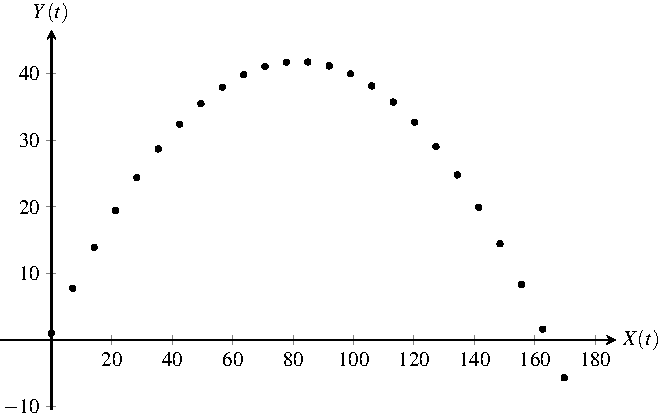
\includegraphics[scale=1.1]{image/13/baseball-trajectory.pdf}
\caption{%%
  The trajectory of the baseball at $t$ seconds after you hit the
  baseball.  The horizontal axis gives the horizontal distance $X(t)$
  between you and the baseball.  You can interpret the horizontal axis
  as representing ground level.  The vertical axis gives the vertical
  distance $Y(t)$ from the baseball to ground level.  All distances
  are in metres.
}
\label{fig:trigonometric:baseball_trajectory}
\end{figure}

\solutionpart{subprob:trigonometric:baseball_trajectory}
\Table{tab:trigonometry:baseball_trajectory} shows the horizontal and
vertical distances of the baseball after you hit the baseball.
\Figure{fig:trigonometric:baseball_trajectory} shows a scatter plot of
values of $X(t)$ versus values of $Y(t)$.  The graph shows that the
baseball reaches a maximum height of approximately $41$~metres above
ground level.  When the baseball is at its maximum height above ground
level, the baseball would be at a horizontal distance of approximately
$80$ metres from you.  When the baseball lands on the ground, the ball
would have covered a horizontal distance of approximately $162$ metres
from where it was hit.

\solutionpart{subprob:trigonometric:baseball_trajectory_30_degree}
At $t$ seconds after you hit the baseball, the vertical distance
between the baseball and ground level can be written as
$Y(t) = -\frac{1}{2}g t^2 + v_y t + h$.  You have the gravitational
constant of $g = 9.8$ metres per second squared, so that
$-\frac{1}{2}g = -\frac{9.8}{2} = -4.9$.  The angle of $\degree{30}$
is equivalent to $\frac{\pi}{6}$ radians, hence you have
$v_y = 50 \sin\frac{\pi}{6}$.  Since
$\sin\frac{\pi}{6} = \frac{1}{2}$, it follows that
$v_y = 50 \times \frac{1}{2} = 25$.  The initial height of the
baseball to ground level is $h = 1$ metre.  Substitute these known
constants into the expression for $Y(t)$ and you obtain
\[
Y(t)
=
-4.9t^2 + 25t + 1.
\]
When $Y(t) = 0$, this means that the baseball has landed on the
ground.  To calculate the values of $t$ such that the expression
$Y(t) = 0$ is true, you must determine the roots of the quadratic
function $f(t) = -4.9t^2 + 25t + 1$.  The discriminant of $f(t)$ is
\[
\Delta
=
25^2 - 4(-4.9)(1)
=
644.6.
\]
Use the quadratic formula to see that the roots of $f(t)$ are
\[
t
=
\frac{
  -25 \pm \sqrt{\Delta}
}{
  2(-4.9)
}
=
\frac{
  -25 \pm \sqrt{\Delta}
}{
  -9.8
}.
\]
One root of $f(t)$ is
\[
t
=
\frac{
  -25 + \sqrt{\Delta}
}{
  -9.8
}
\approx
-0.039691
\]
which is negative so you may reject this root as non-sense in the
context of the problem.  The other root of $f(t)$ is
%%
\begin{equation}
\label{eqn:trigonometric:baseball_30_degree_root}
\begin{aligned}
t
&=
\frac{
  -25 - \sqrt{\Delta}
}{
  -9.8
} \\[4pt]
&\approx
5.141732.
\end{aligned}
\end{equation}
%%
That is, after you hit the baseball you must wait approximately
$5.14$ seconds for the baseball to land on the ground.

At $t$ seconds after you hit the baseball, the horizontal
distance~(metres) from the baseball to its original position can be
written as $X(t) = v_x t$.  You have
\[
v_x
=
50 \cos\frac{\pi}{6}
=
50 \times \frac{\sqrt{3}}{2}
=
25\sqrt{3}
\]
and hence $X(t) = 25\sqrt{3} t$.  The exact time at which the baseball
lands on the ground is given by
\Equation{eqn:trigonometric:baseball_30_degree_root}.  Use
\Equation{eqn:trigonometric:baseball_30_degree_root} to write
\[
X(t)
=
\frac{
  25\sqrt{3} (-25 - \sqrt{\Delta})
}{
  -9.8
}
\approx
222.643528.
\]
That is, when the baseball lands on the ground the ball would be a
horizontal distance of approximately $222.64$ metres away from its
original position.
\end{solution}
}{}

\item High and low tides in Geelong.  See also page~94 of the
  following book: W.~T.~Griffith and J.~W.~Brosing.  \emph{The Physics
    of Everyday Phenomena: A Conceptual Introduction to Physics}.
\ifbool{showSolution}{
\begin{solution}

\end{solution}
}{}

\begin{table}[!htbp]
\centering
\begin{tabular}{ccccccccccccc} \toprule
Month & Jan & Feb & Mar & Apr & May & Jun & Jul & Aug & Sep & Oct & Nov & Dec \\
Mean  & 8.9 & 8.1 & 7.3 & 5.5 & 4   & 3.5 & 3.9 & 4.5 & 5.9 & 6.5 & 7.4 & 7.5 \\\bottomrule
\end{tabular}

\caption{%%
  The mean daily number of hours of sunshine for the city of
  Melbourne, Victoria, Australia.  The mean for each month was
  calculated using data for the years from $1961$ to $1990$.  The mean
  values are provided by the United Nations.
}
\label{tab:trigonometric:mean_daily_sunshine}
\end{table}

\item\emph{Hours of sunshine.}
  \Table{tab:trigonometric:mean_daily_sunshine} shows the mean
  daily number of hours of sunshine for Melbourne for each month of
  the year.\footnote{
    The data are available at
    \url{http://web.archive.org/web/20180712183444/http://data.un.org/Data.aspx?d=CLINO\&f=ElementCode\%3a15\%3bCountryCode\%3aAU\&c=2,5,6,7,10,15,18,19,20,22,24,26,28,30,32,34,36,38,40,42,44,46\&s=CountryName:asc,WmoStationNumber:asc,StatisticCode:asc\&v=1},
    accessed 2018-07-12.
  }
  %%
  \begin{packedenum}
  \item\label{subprob:trigonometric:mean_daily_sunshine_graph}
    As in \Part{subeg:trigonometric:mean_max_temperature_graph} of
    \Example{eg:trigonometric:mean_maximum_temperature}, associate the
    months with equally spaced values between $0$ and $2\pi$.  Produce
    a scatter plot of the data in
    \Table{tab:trigonometric:mean_daily_sunshine}.  The horizontal
    axis should represent a time of the year and the vertical axis the
    mean daily number of hours of sunshine.  Explain what you notice
    about the graph.

  \item\label{subprob:trigonometric:mean_daily_sunshine_model}
    Suppose the data in \Table{tab:trigonometric:mean_daily_sunshine}
    can be modelled as a function of the form
    %%
    \begin{equation}
    \label{eqn:trigonometric:mean_daily_sunshine_c1}
    f(x)
    =
    a \cos(cx) + b
    \end{equation}
    %%
    where the parameters $\triple{a}{b}{c}$ are to be estimated from
    the data.  You may assume that $c = 1$ and that $f(x)$ has a
    period of $2\pi$.  Use the given data to estimate the values of
    the parameters $a$ and $b$.  Graph your function $f(x)$ together
    with the scatter plot
    from \Part{subprob:trigonometric:mean_daily_sunshine_graph}.
    Calculate the root mean square error~(RMSE) and coefficient of
    determination $R^2$ of $f(x)$.  Based on the RMSE and $R^2$,
    explain how well the function $f(x)$ models the data in
    \Table{tab:trigonometric:mean_daily_sunshine}.

  \item\label{subprob:trigonometric:mean_daily_sunshine_compress}
    The graph
    from \Part{subprob:trigonometric:mean_daily_sunshine_model} seems
    to suggest that you can compress the graph of $f(x)$ along the
    horizontal axis in order to better fit the given data.  In other
    words, increasing the value of $c$ in
    \Equation{eqn:trigonometric:mean_daily_sunshine_c1}, while keeping
    the values of $a$ and $b$ constant, might result in a better fit
    to the data in \Table{tab:trigonometric:mean_daily_sunshine}.
    Create a table that has three columns and as many rows as
    necessary.  Going from left to right, the first column should have
    the header ``$c$'' and lists increasing values of $c$ from $1$ up
    to and including $1.1$.  The value of $c$ increments by $0.01$ so
    going down the rows you would have $1$, $1.01$, $1.02$, and so on,
    up to $1.1$.  The second column should have the header ``RMSE''
    and lists the root mean square error corresponding to each value
    of $c$.  Finally, the third column should have the header
    ``$R^2$'' and lists the coefficient of determination corresponding
    to each value of $c$.  On the same set of axes, graph the values
    of $c$ versus the RMSE and the values of $c$ versus $R^2$.  Using
    your table and the graph, explain what you notice about the values
    of the RMSE and $R^2$ as $c$ increases.  Which value of $c$ would
    result in \Equation{eqn:trigonometric:mean_daily_sunshine_c1}
    having the smallest RMSE and largest $R^2$?

  \item\label{subprob:trigonometric:mean_daily_sunshine_remove_highest}
    Note that in the graph
    of \Part{subprob:trigonometric:mean_daily_sunshine_model} you may
    ignore the highest mean daily number of hours of sunshine and fit
    a cosine function to the remaining data.  That is, suppose that
    you ignore the data for January in
    \Table{tab:trigonometric:mean_daily_sunshine}.  Suppose that in
    \Equation{eqn:trigonometric:mean_daily_sunshine_c1} you set
    $c = 1$.  Estimate the values of the parameters $a$ and $b$ by
    using the data from February onwards.  Using the estimated values
    for the parameters $\triple{a}{b}{c}$ calculate the RMSE and $R^2$
    of $f(x)$.  Now as
    in \Part{subprob:trigonometric:mean_daily_sunshine_compress},
    suppose that you keep the values of $a$ and $b$ constant and vary
    the value of $c$.  Create a table as
    in \Part{subprob:trigonometric:mean_daily_sunshine_compress} with
    the value of $c$ increasing from $1$ up to $1.15$ by an increment
    of $0.01$.  Using the values in your table, graph on one set of
    axes the values of $c$ versus the RMSE and the values of $c$
    versus $R^2$.  Explain what you notice about the values of the
    RMSE and $R^2$ as $c$ increases.  Which value of $c$ would result
    in \Equation{eqn:trigonometric:mean_daily_sunshine_c1} having the
    smallest RMSE and largest $R^2$?

  \item\label{subprob:trigonometric:mean_daily_sunshine_best_model}
    Let $f(x)$ be the function
    from \Part{subprob:trigonometric:mean_daily_sunshine_compress}
    that best fits the given data set.  That is, $f(x)$ has the lowest
    RMSE and highest $R^2$ of such values
    from \Part{subprob:trigonometric:mean_daily_sunshine_compress}.
    Furthermore, let $g(x)$ be the function
    from \Part{subprob:trigonometric:mean_daily_sunshine_remove_highest}
    that best fits the given data set.  On the same set of axes, graph
    the data in \Table{tab:trigonometric:mean_daily_sunshine} and the
    functions $f(x)$ and $g(x)$.  Use the values of the RMSE and $R^2$
    to help you decide which of the two functions is better than the
    other at modelling the given data.

  \item\label{subprob:trigonometric:mean_daily_sunshine_other_model}
    {\color{red}
      Explain another way to improve the fit of $f(x)$ to the given
      data.
    }
  \end{packedenum}
\ifbool{showSolution}{
\begin{solution}
\solutionpart{subprob:trigonometric:mean_daily_sunshine_graph}
\Figure{fig:trigonometric:mean_daily_sunshine} shows a scatter plot of
the data in \Table{tab:trigonometric:mean_daily_sunshine}.  As the
figure shows, the black dots seem to follow the graph of a cosine
function.  This suggests that you can model the given data as a
function of the form $f(x) = a \cos(cx) + b$, where the parameters
$\triple{a}{b}{c}$ are to be estimated from the data.  Here, $x$
represents a time of the year and $f(x)$ represents the mean daily
number of hours of sunshine corresponding to $x$.

\begin{figure}[!htbp]
\centering
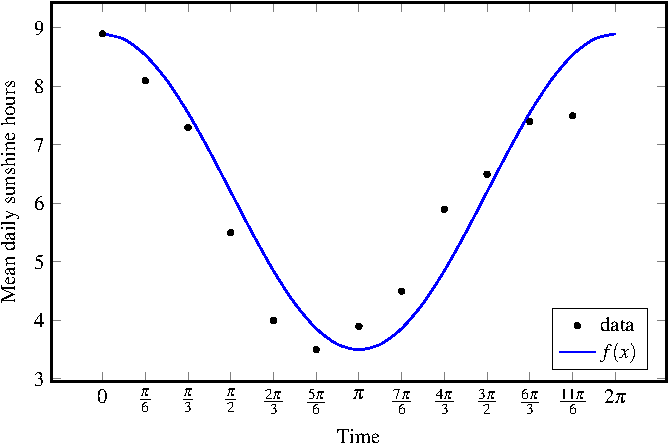
\includegraphics[scale=1.1]{image/13/mean-daily-sunshine.pdf}
\caption{%%
  The mean daily number of hours of sunshine for Melbourne.  The
  horizontal axis represents time of the year.  So $0$ corresponds to
  January, $\frac{\pi}{6}$ corresponds to February, and so on.  The
  black dots show the data in
  \Table{tab:trigonometric:mean_daily_sunshine}.  The blue curve is a
  graph of the prediction function $f(x)$ as defined by
  \Equation{eqn:trigonometric:mean_daily_sunshine}.
}
\label{fig:trigonometric:mean_daily_sunshine}
\end{figure}

\solutionpart{subprob:trigonometric:mean_daily_sunshine_model}
The value $b$ of the midline is the mean of the lowest and highest
values in \Table{tab:trigonometric:mean_daily_sunshine}.  The minimum
and maximum values in the table are $3.5$ and $8.9$, respectively,
hence the value of the midline is
\[
b
=
\frac{3.5 + 8.9}{2}
=
6.2.
\]
The amplitude $a$ is the absolute value of the difference between the
highest value in \Table{tab:trigonometric:mean_daily_sunshine} and the
value of the midline.  So you have
\[
a
=
\absoluteValue{8.9 - 6.2}
=
\absoluteValue{2.7}
=
2.7.
\]
Since you have assumed that $c = 1$, it follows that the function
$f(x)$ can be written as
%%
\begin{equation}
\label{eqn:trigonometric:mean_daily_sunshine}
f(x)
=
2.7 \cos x + 6.2
\end{equation}
%%
which is graphed in \Figure{fig:trigonometric:mean_daily_sunshine}.
The function $f(x)$ has a root mean square error~(RMSE) of
$\text{RMSE} \approx 0.609530$ and a coefficient of determination of
$R^2 \approx 0.876352$.  The value of the RMSE means that on average
the prediction of $f(x)$ differs from the data by approximately $0.6$
hours.  The value of $R^2$ suggests that $f(x)$ models the given data
very well.  However, a model whose value of $R^2$ is close to $0.9$ or
higher would be better than $f(x)$.

\begin{table}[!htbp]
\centering
\begin{tabular}{ccc} \toprule
$c$    & RMSE       & $R^2$      \\\midrule
$1.00$ & $0.609530$ & $0.876352$ \\
$1.01$ & $0.589218$ & $0.884456$ \\
$1.02$ & $0.574005$ & $0.890345$ \\
$1.03$ & $0.563949$ & $0.894154$ \\
$1.04$ & $0.558963$ & $0.896017$ \\
$1.05$ & $0.558812$ & $0.896073$ \\
$1.06$ & $0.563137$ & $0.894458$ \\
$1.07$ & $0.571484$ & $0.891306$ \\
$1.08$ & $0.583350$ & $0.886746$ \\
$1.09$ & $0.598218$ & $0.880899$ \\
$1.10$ & $0.615595$ & $0.873879$ \\\bottomrule
\end{tabular}

\caption{%%
  Consider the function $f(x) = 2.7 \cos(cx) + 6.2$.  Increasing the
  value of $c$ has the effect of changing the values of the root mean
  square error~(RMSE) and the coefficient of determination of $f(x)$.
}
\label{tab:trigonometric:mean_daily_sunshine_vary_c}
\end{table}

\begin{figure}[!htbp]
\centering
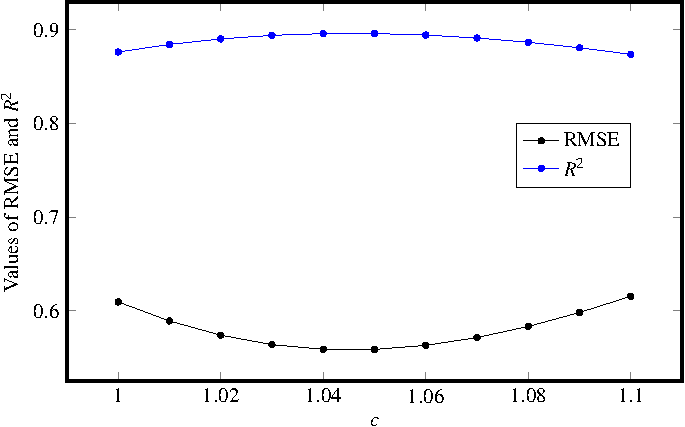
\includegraphics[scale=1.1]{image/13/sunshine-vary-c.pdf}
\caption{%%
  Suppose in \Equation{eqn:trigonometric:mean_daily_sunshine_c1} that
  $a = 2.7$ and $b = 6.2$.  Increasing the value of $c$ has the effect
  of changing the values of the RMSE and $R^2$ of $f(x)$.
}
\label{fig:trigonometric:mean_daily_sunshine_vary_c}
\end{figure}

\solutionpart{subprob:trigonometric:mean_daily_sunshine_compress}
Suppose you leave the constants $a = 2.7$ and $b = 6.2$ in
\Equation{eqn:trigonometric:mean_daily_sunshine_c1} alone, but only
change the value of $c$.
\Table{tab:trigonometric:mean_daily_sunshine_vary_c} shows that
increasing the value of $c$ affects how well $f(x)$ models the given
data set.  As the value of $c$ increases from $1$ up to $1.1$, the
RMSE decreases from approximately $0.6095$ down to approximately
$0.5588$ and then increases to $0.6156$.  Furthermore, the value of
$R^2$ increases from approximately $0.8764$ up to $0.8961$ and then
decreases to $0.8739$.  The data in
\Table{tab:trigonometric:mean_daily_sunshine_vary_c} are graphed in
\Figure{fig:trigonometric:mean_daily_sunshine_vary_c}.  Among the
values of $c$ listed in
\Table{tab:trigonometric:mean_daily_sunshine_vary_c}, the value
$c = 1.05$ results in the lowest value of the root mean square error
at $\text{RMSE} \approx 0.558812$ and highest value of the coefficient
of determination at $R^2 \approx 0.896073$.  You may conclude that if
in \Equation{eqn:trigonometric:mean_daily_sunshine_c1} you have
$a = 2.7$, $b = 6.2$, and $c \approx 1.05$ then $f(x)$ would model the
data in \Table{tab:trigonometric:mean_daily_sunshine} very well.

\begin{table}[!htbp]
\centering
\begin{tabular}{ccc} \toprule
$c$    & RMSE       & $R^2$      \\\midrule
$1.00$ & $0.608533$ & $0.876756$ \\
$1.01$ & $0.572170$ & $0.891045$ \\
$1.02$ & $0.538615$ & $0.903450$ \\
$1.03$ & $0.508211$ & $0.914043$ \\
$1.04$ & $0.481317$ & $0.922899$ \\
$1.05$ & $0.458297$ & $0.930098$ \\
$1.06$ & $0.439491$ & $0.935717$ \\
$1.07$ & $0.425185$ & $0.939834$ \\
$1.08$ & $0.415572$ & $0.942524$ \\
$1.09$ & $0.410721$ & $0.943858$ \\
$1.10$ & $0.410555$ & $0.943903$ \\
$1.11$ & $0.414860$ & $0.942721$ \\
$1.12$ & $0.423307$ & $0.940364$ \\
$1.13$ & $0.435493$ & $0.936881$ \\
$1.14$ & $0.450986$ & $0.932311$ \\
$1.15$ & $0.469360$ & $0.926682$ \\\bottomrule
\end{tabular}

\caption{%%
  Consider the function $f(x) = 2.3 \cos(cx) + 5.8$.  Increasing the
  value of $c$ has the effect of changing the values of the root mean
  square error~(RMSE) and the coefficient of determination of $f(x)$.
}
\label{tab:trigonometric:mean_daily_sunshine_vary_c_ignore_highest}
\end{table}

\begin{figure}[!htbp]
\centering
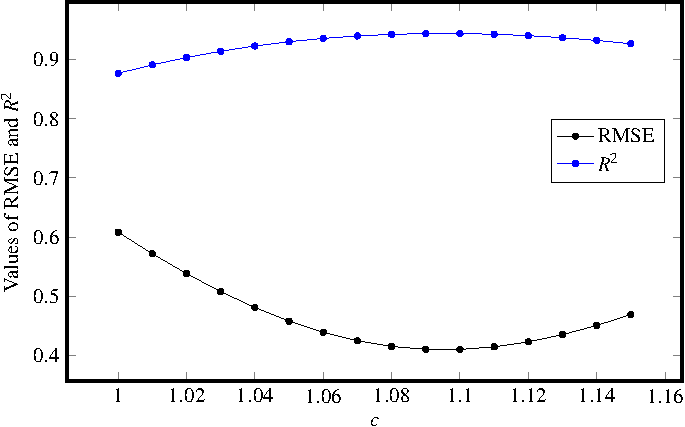
\includegraphics[scale=1.1]{image/13/sunshine-vary-c-ignore-highest.pdf}
\caption{%%
  Suppose that you model the data in
  \Table{tab:trigonometric:mean_daily_sunshine} as the cosine function
  $f(x) = 2.3 \cos(cx) + 5.8$.  Increasing the value of $c$ affects
  how well $f(x)$ models the given data.
}
\label{fig:trigonometric:mean_daily_sunshine_vary_c_ignore_highest}
\end{figure}

\solutionpart{subprob:trigonometric:mean_daily_sunshine_remove_highest}
First, you estimate the value of $b$.  The value of the midline is the
mean of the lowest and highest values in
\Table{tab:trigonometric:mean_daily_sunshine}, while ignoring the data
column for January.  The minimum and maximum values are $3.5$ and
$8.1$, respectively, hence you have
\[
b
=
\frac{3.5 + 8.1}{2}
=
5.8
\]
and so the value of the amplitude is
\[
a
=
\absoluteValue{8.1 - 5.8}
=
\absoluteValue{2.3}
=
2.3.
\]
Thus you have the function $f(x) = 2.3 \cos(cx) + 5.8$.
\Table{tab:trigonometric:mean_daily_sunshine_vary_c_ignore_highest}
shows that increasing the value of $c$ affects how well $f(x)$ models
the given data set.  As $c$ increases from $1$ up to $1.15$, the value
of the RMSE decreases from approximately $0.608533$ down to
approximately $0.410555$ and then increases to $0.469360$.
Furthermore, the value of $R^2$ increases from approximately
$0.876756$ up to about $0.943903$ and then decreases to $0.926682$.
The data in
\Table{tab:trigonometric:mean_daily_sunshine_vary_c_ignore_highest}
are graphed in
\Figure{fig:trigonometric:mean_daily_sunshine_vary_c_ignore_highest}.
As the data table and the figure show, if $c \approx 1.1$ then $f(x)$
attains its lowest value of RMSE at approximately $0.410555$ and
highest value of $R^2$ at approximately $0.943903$.

\begin{figure}[!htbp]
\centering
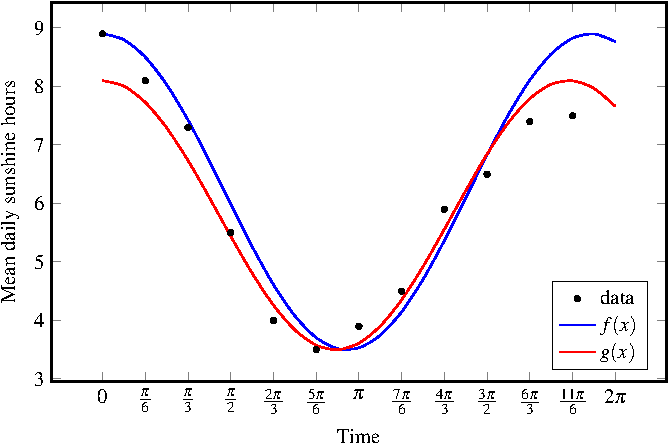
\includegraphics[scale=1.1]{image/13/mean-daily-sunshine-models.pdf}
\caption{%%
  Comparison of data and prediction for the mean daily number of hours
  of sunshine in Melbourne.  The black dots show the data in
  \Table{tab:trigonometric:mean_daily_sunshine}.  The blue and red
  curves are graphs of
  \Equations{eqn:trigonometric:mean_daily_sunshine_f(x)}{eqn:trigonometric:mean_daily_sunshine_g(x)},
  respectively.
}
\label{fig:trigonometric:mean_daily_sunshine_models}
\end{figure}

\solutionpart{subprob:trigonometric:mean_daily_sunshine_best_model}
From \Part{subprob:trigonometric:mean_daily_sunshine_compress},
the model that best fits the given data is
%%
\begin{equation}
\label{eqn:trigonometric:mean_daily_sunshine_f(x)}
f(x)
=
2.7 \cos(1.05 x) + 6.2
\end{equation}
%%
and
from \Part{subprob:trigonometric:mean_daily_sunshine_remove_highest},
the corresponding best model is
%%
\begin{equation}
\label{eqn:trigonometric:mean_daily_sunshine_g(x)}
g(x)
=
2.3 \cos(1.1 x) + 5.8.
\end{equation}
%%
Both functions are graphed in
\Figure{fig:trigonometric:mean_daily_sunshine_models} together with
the given data set.  The RMSE of $g(x)$ is smaller than that of
$f(x)$.  Furthermore, the value of $R^2$ of $g(x)$ is higher than that
of $f(x)$.  Based on the values of the RMSE and $R^2$, you may
conclude that $g(x)$ is better than $f(x)$ at modelling the mean daily
number of hours of sunshine in Melbourne.
\end{solution}
}{}

\begin{figure}[!htbp]
\centering
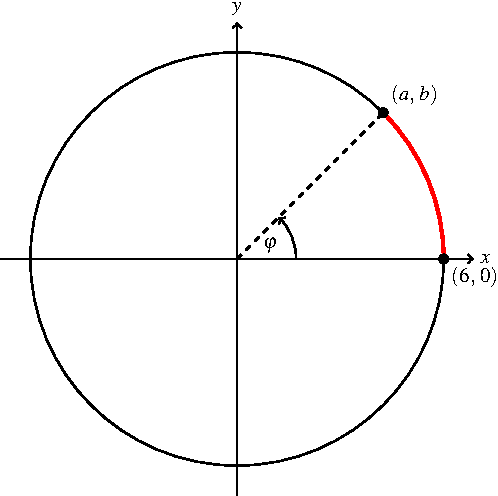
\includegraphics[scale=1.1]{image/13/ant-circle.pdf}
\caption{%%
  An ant starts at the point $\tuple{6}{0}$.  It travels at a constant
  speed along the edge of a Blu-ray disc that has a radius of $r = 6$
  centimetres.  The disc is interpreted as a circle that is centred at
  the origin.  If the ant stops at the point $\tuple{a}{b}$, the path
  of the ant is represented by the red arc.
}
\label{fig:trigonometric:ant_on_disc}
\end{figure}

\item\emph{Ant on a disc.}
  A Blu-ray disc has a radius of $6$ centimetres.  An ant travels at a
  constant speed along the edge of the disc.  Suppose that the centre
  of the disc is at the origin $\tuple{0}{0}$ of the Cartesian
  coordinate system.  At any time the position of the ant along the
  edge of the disc can be illustrated as in
  \Figure{fig:trigonometric:ant_on_disc}.
  %%
  \begin{packedenum}
  \item\label{subprob:trigonometric:ant_distance}
    The ant is initially at the point $\tuple{6}{0}$  in
    \Figure{fig:trigonometric:ant_on_disc}.  It walks all the way
    around the edge of the disc and returns to its starting position.
    Calculate the distance~(centimetres) that the ant travelled.

  \item\label{subprob:trigonometric:ant_time}
    If the ant travelled a distance of $d > 0$ centimetres at a
    constant speed of $v > 0$ centimetres per second, the total amount
    of time $T$ required to cover the given distance is $T = d / v$
    seconds.  Suppose that the ant runs at a constant speed of $2$
    centimetres per second.  How much time is required for the ant to
    go around the edge of the disc once?

  \item\label{subprob:trigonometric:ant_speed}
    In $18$ seconds the ant makes $3$ complete trips around the edge
    of the disc.  Calculate the speed of the ant.

  \item\label{subprob:trigonometric:ant_angle}
    Suppose that the ant is originally at the point $\tuple{6}{0}$ in
    \Figure{fig:trigonometric:ant_on_disc}.  It travels a distance of
    $d$ centimetres along the edge of the disc and makes an angle of
    $\varphi$ radians with respect to the positive half of the
    horizontal axis.  As the radius of the disc is $r = 6$
    centimetres, the angle $\varphi$ can be written in terms of the
    radius and distance as
    \[
    \varphi
    =
    \frac{d}{6}.
    \]
    If the ant travels a distance of $\pi$ centimetres along the edge
    of the disc, calculate the angle between the ant and the positive
    half of the horizontal axis.  If the ant travels a distance of $d$
    centimetres along the edge of the disc and makes an angle of
    $\degree{75}$ with respect to the positive half of the horizontal
    axis, how far in centimetres did the ant travel?

  \item\label{subprob:trigonometric:ant_x_y_distances}
    The ant starts at the point $\tuple{6}{0}$, travels along the edge
    of the disc, and stops at the point $\tuple{a}{b}$ as shown in
    \Figure{fig:trigonometric:ant_on_disc}.  Write an expression for
    each of $a$ and $b$ in terms of trigonometric functions.
  \end{packedenum}
\ifbool{showSolution}{
\begin{solution}
\solutionpart{subprob:trigonometric:ant_distance}
Assume that the ant makes one full trip around the edge of the disc.
The distance that the ant travelled is equivalent to the circumference
of the disc.  Since the disc has a radius of $6$ centimetres, the
circumference of the disc is
\[
2\pi \times 6
=
12\pi
\approx
37.6991
\]
centimetres.  If the ant makes one complete trip around the edge of
the disc, then it would have travelled a distance of approximately
$37.6991$~cm.

\solutionpart{subprob:trigonometric:ant_time}
Suppose that the ant runs around the edge of the disc once.  You know
from \Part{subprob:trigonometric:ant_distance} that the distance the
ant covers would be $d = 12\pi$ centimetres.  Since the ant runs at a
constant speed of $v = 2$ centimetres per second, the time required to
complete one trip around the edge of the disc is
\[
T
=
\frac{12\pi}{2}
=
6\pi
\approx
18.8496
\]
seconds.

\solutionpart{subprob:trigonometric:ant_speed}
If the ant requires $18$ seconds to make $3$ complete trips around the
edge of the disc, then each complete trip requires
$18 / 3 = 6$ seconds.  That is, in $6$ seconds the ant covers a
distance of $12\pi$ centimetres.  If $v$ is the speed~(cm per second)
of the ant, then the total time can be written as
$6 = \frac{12\pi}{v}$.  Multiply both sides by $v$ to get
$6v = 12\pi$.  Now divide both sides by $6$ to get
$v = \frac{12\pi}{6}$, which can be simplified to
$v = 2\pi \approx 6.2832$.  Thus the speed of the ant is approximately
$6.2832$ centimetres per second.

The speed of the ant can also be calculated as follows.  Each complete
trip around the edge of the disc translates to $12\pi$ centimetres.
So $3$ complete trips would mean that the ant covers a total distance
of $3 \times 12\pi = 36\pi$ centimetres.  If $v$ is the speed~(cm per
second) of the ant, the time required to complete $3$ trips can be
written as $18 = \frac{36\pi}{v}$.  Solve for $v$ to get
$v = \frac{36\pi}{18} = 2\pi$, which is the same as above.

\solutionpart{subprob:trigonometric:ant_angle}
The ant starts at the point $\tuple{6}{0}$ and travels a distance of
$d = \pi$ centimetres along the edge of the disc.  The angle $\varphi$
that the ant makes with respect to the positive half of the horizontal
axis can be written as $\varphi = \frac{\pi}{6}$ radians, which is
equivalent to $\degree{30}$.

Suppose that the ant starts at the point $\tuple{6}{0}$.  It travels a
distance of $d$ centimetres along the edge of the disc and makes an
angle of $\degree{75}$ with respect to the positive half of the
horizontal axis.  You can write the given angle as
$\degree{75} = \degree{30} + \degree{45}$.  You know that
$\degree{30}$ and $\degree{45}$ are equivalent to $\frac{\pi}{6}$ and
$\frac{\pi}{4}$ radians, respectively.  Then $\degree{75}$ is
equivalent to
\[
\frac{\pi}{6} + \frac{\pi}{4}
=
\frac{2\pi}{12} + \frac{3\pi}{12}
=
\frac{5\pi}{12}
\]
radians.  The distance travelled can be written in terms of the angle
as the expression $\frac{5\pi}{12} = \frac{d}{6}$.  Solve for $d$ and
simplify to get
\[
d
=
\frac{6 \times 5\pi}{12}
=
\frac{5\pi}{2}
\approx
7.853982.
\]
Thus the ant travelled a distance of approximately $7.85$
centimetres.

\begin{figure}[!htbp]
\centering
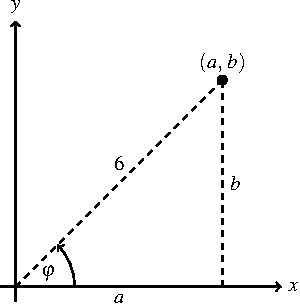
\includegraphics[scale=1.1]{image/13/right-triangle.pdf}
\caption{%%
  The coordinate $\tuple{a}{b}$ of the ant can be visualised as a
  point on a right-angled triangle.
}
\label{fig:trigonometric:ant_coordinate}
\end{figure}

\solutionpart{subprob:trigonometric:ant_x_y_distances}
The coordinate $\tuple{a}{b}$ of the ant can be interpreted as a point
on a right-angled triangle, as shown in
\Figure{fig:trigonometric:ant_coordinate}.  Note that you have the
expression $\cos\varphi = \frac{a}{6}$, which can be solved for $a$ to
get $a = 6 \cos\varphi$.  Furthermore, you have
$\sin\varphi = \frac{b}{6}$ and solving for $b$ results in
$b = 6 \sin\varphi$.
\end{solution}
}{}

\item Rolling motion.  See pages~267--269 of the book:
  N.~J.~Giordano.  \emph{College Physics: Reasoning and Relationships}.
\ifbool{showSolution}{
\begin{solution}

\end{solution}
}{}

\item The physics of waves.  See chapter~15 of the book:
  W.~T.~Griffith and J.~W.~Brosing.  \emph{The Physics of Everyday
    Phenomena: A Conceptual Introduction to Physics}.
\ifbool{showSolution}{
\begin{solution}

\end{solution}
}{}

\item Simple harmonic motion and damped motion.  See page~287 of the
  book: M.~Sullivan.  \emph{Trigonometry: A Unit Circle Approach}.
  See also chapter~11 of the book:  N.~J.~Giordano.
  \emph{College Physics: Reasoning and Relationships}.
\ifbool{showSolution}{
\begin{solution}

\end{solution}
}{}

\item Sound.  See chapter~13 of the book:  N.~J.~Giordano.
  \emph{College Physics: Reasoning and Relationships}.
\ifbool{showSolution}{
\begin{solution}

\end{solution}
}{}
\end{problem}

\end{document}
